\documentclass[11pt,twoside,openright,a4paper]{book}

%%%%%%%%%%  paquetes incluidos  %%%%%%%%%%
\usepackage[latin1]{inputenc}
\usepackage[english,spanish]{babel}
\usepackage{fancyhdr}
\usepackage{minitoc}
\usepackage{epsfig}
\usepackage{url}

%%%%%%  Medidas del documento  %%%%%%
\textheight = 23 cm
\textwidth  = 16 cm
\hoffset    = 0 cm
\voffset    = -2.5 cm
\oddsidemargin =  0.0 cm
\evensidemargin =  0.0 cm
\topmargin  = 2.5 cm

%%%%%%%  formateo del encabezado y pie de pagina  %%%%%%%%%%%
\pagestyle{fancy}

%\addtolength{\headwidth}{\marginparsep}
%\addtolength{\headwidth}{\marginparwidth}
\renewcommand{\chaptermark}[1]{\markboth{\MakeUppercase\chaptername\ \thechapter.\ #1}{}}
\renewcommand{\sectionmark}[1]{\markright{\thesection\ #1}}
\fancyhf{}
\fancyhead[LE,RO]{\bfseries\thepage}
\fancyhead[LO]{\bfseries\rightmark}
\fancyhead[RE]{\bfseries\leftmark}
\fancypagestyle{pain}{
	\fancyhead{} % consigue el librado de cabeceras
        \renewcommand{\headrulewidth}{Opt}  % y la linea
}

% para pagina posterior en blanco
\newcommand{\clearemptydoublepage}{\newpage{\pagestyle{empty}\cleardoublepage}}
\clearemptydoublepage

%%%%%%%%%%  comienzo del documento  %%%%%%%%%%
\begin{document}

%%%%%%%%%%  formato de la portada %%%%%%%%%%
%\frontmatter
\newlength{\centeroffset} \setlength{\centeroffset}{-0.5\oddsidemargin} %
%\addtolength{\centeroffset}{0.5\evensidemargin}
\thispagestyle{empty} \vspace*{\stretch{1}} \hspace*{\centeroffset} \noindent
\begin{minipage}{\textwidth}
\flushright{\Huge \bf  Cluster Heterog�neo De Computadoras} \noindent
\rule[-1ex]{\textwidth}{5pt}\\[4.5ex]
\end{minipage}
\vspace{\stretch{1}} \noindent \hspace*{\centeroffset}
\begin{minipage}{\textwidth}
\flushright{\bfseries   EMILIO JOS� PLAZA NIETO\\[1.5ex]}
\today
\end{minipage}
\endinput

\clearemptydoublepage

%%%%%%%%%% formateo y generaci�n del indice  %%%%%%%%%%
\dominitoc
\tableofcontents
\clearemptydoublepage
\listoffigures
\clearemptydoublepage

%%%%%%%%%% inclusion de los distintos temas q constituyen el documento  %%%%%%%%%%
\chapter{INTRODUCCI�N.}
\minitoc
\section{Resumen proyecto.}
Debido al espectacular auge de la tecnolog�a y de la inform�tica en la actualidad los equipos inform�ticos
se quedan anticuados en un plazo corto de tiempo. Para aprovechar estos ``viejos'' equipos se puede construir un
cluster\footnote{conjunto de computadoras interconectadas con dispositivos de alta velocidad que act�an en
conjunto usando el poder c�mputo de varios CPU en combinaci�n para resolver ciertos problemas dados}, de
forma que la capacidad de computaci�n que obtengamos pueda llegar a compensarnos ante la inversi�n a realizar
en equipos m�s potentes. Programas con gran carga de computaci�n tardar�an bastante tiempo en realizarse
en uno de estos ``viejos'' ordenadores. Se pretende usar estos ordenadores para construir un cluster y con �l
reducir este tiempo de computaci�n mediante el reparto de la carga entre sus nodos.
	
Este proyecto se basa en el desarrollo de un cluster de computadoras heterog�neo formado por un
front-end\footnote{ordenador central o servidor encargado de gestionar los nodos y operaciones que se
realizan en el cluster} y veinte y tres nodos.

La realizaci�n de este cluster de computadoras heterog�neo estar� compuesta de dos fases, una de configuraci�n
hardware y otra de desarrollo software. La configuraci�n hardware estar� a su vez dividida en tres partes, configuraci�n
del equipo central o front-end, configuraci�n de los respectivos nodos que formar�n parte del cluster y configuraci�n
de la red de interconexi�n.

La configuraci�n software consistir� en la realizaci�n de programas para control de latencia de red y
ancho de banda de la misma, adem�s de un programa para obtener el incremento de rendimiento o ganancia de velocidad
que se consigue a�adiendo nuevos nodos a la resoluci�n del problema.

Adem�s, se instalar�n programas que nos permitir�n observar los detalles de utilizaci�n de cada nodo:
n�meros de usuarios conectados al nodo, memoria libre, memoria swap disponible, etc.

\section{Memoria descriptiva.}
Instalaci�n m�nima del sistema operativo en cada uno de los nodos, es decir, se instalar� los servicios
m�nimos para realizar un procesamiento paralelo y servicios de acceso para que el sistema funcione correctamente.
Adem�s se recompilar� el n�cleo del sistema operativo.

Configuraci�n de la red de interconexi�n entre los nodos y el ordenador central o front-end a trav�s del
protocolo DHCP (Dinamic Host Configure Protocol) de forma que el ordenador central sea el encargado
de asignar la direcci�n IP correspondiente a cada nodo, en funci�n de la direcci�n MAC (Medium Access Control)
de la tarjeta de red Ethernet.

Configuraci�n de un firewall en la m�quina central o front-end que permita �nicamente el acceso desde
el exterior a �ste a trav�s del protocolo SSH Secure SHell.

Los nodos a�adidos se configurar�n de forma que puedan arrancar v�a NFS (Network File System) a
trav�s del protocolo DHCP, obteniendo su direcci�n IP mediante el protocolo DHCP cuando el nodo arranque de
forma local.

Instalaci�n del software PVM (Parallel Virutal Machine) y XPVM (A Graphical Console and Monitor for
PVM). Configuraci�n de dicho software, de forma que permita la ejecuci�n de programas paralelos basados en el
reparto de la carga computacional mediante paso de mensajes entre los distintos nodos del cluster.

Instalaci�n y configuraci�n del software LAM/MPI (Local Area Multicomputer/Message Passing Interface)
con el mismo prop�sito que PVM. Se realizar�n comparativas entre ambos paquetes a trav�s de la implementaci�n
de programas.

Instalaci�n de herramientas software que nos permitan observar el estado del cluster.

\section{Planificaci�n.}
Se realizar� un estudio sobre qu� distribuci�n Linux se ajusta mejor a nuestras necesidades en funci�n
de los ordenadores que disponemos para realizar el cluster.

Instalaci�n m�nima distribuci�n Linux en el front-end y recompilaci�n del n�cleo.
	
Configuraci�n protocolo DHCP.
	
Configuraci�n de un firewall en la m�quina central o front-end.
	
Instalaci�n y configuraci�n de PVM y XPVM. Desarrollo de programas en PVM.
	
Instalaci�n y configuraci�n de LAM/MPI. Desarrollo de programas en LAM/MPI.
	
Instalaci�n de herramientas software para conocer el estado del ordenador central y los restantes nodos.

\section{Introducci�n a los cluster de computadoras.}
\subsection{�Que es un cluster de computadoras?}
Un cluster es un grupo de equipos independientes que ejecutan una serie de aplicaciones de forma
conjunta y aparecen ante clientes y aplicaciones como un solo sistema. Los clusters permiten aumentar la
escalabilidad, disponibilidad y fiabilidad de m�ltiples niveles de red.

La escalabilidad es la capacidad de un equipo para hacer frente a vol�menes de trabajo cada vez mayores
sin, por ello, dejar de prestar un nivel de rendimiento aceptable. Existen dos tipos de escalabilidad:
\begin{itemize}
\item Escalabilidad del hardware (tambi�n denominada �escalamiento vertical�). Se basa en la
utilizaci�n de un gran equipo cuya capacidad se aumenta a medida que lo exige la carga de trabajo existente.
\item Escalabilidad del software (tambi�n denominada �escalamiento horizontal�). Se basa, en
cambio, en la utilizaci�n de un cluster compuesto de varios equipos de mediana potencia que funcionan en t�ndem de
forma muy parecida a como lo hacen las unidades de un RAID (Redundant Array of Inexpensive Disks o Array
redundante de discos de bajo coste). Se utilizan el t�rmino RAC (Redundant Array of Computers o Array redundante
de equipos) para referirse a los clusters de escalamiento horizontal. Del mismo modo que se a�aden discos a
un array RAID para aumentar su rendimiento, se pueden a�adir nodos a un cluster para aumentar tambi�n su
rendimiento.
\end{itemize}

La disponibilidad y la fiabilidad son dos conceptos que, si bien se encuentran �ntimamente relacionados,
difieren ligeramente. La disponibilidad es la calidad de estar presente, listo para su uso, a mano, accesible;
mientras que la fiabilidad es la probabilidad de un funcionamiento correcto.

Pero hasta el m�s fiable de los equipos acaba fallando. Los fabricantes de hardware intentan anticiparse
a los fallos aplicando la redundancia en �reas clave como son las unidades de disco, las fuentes de alimentaci�n,
las controladoras de red y los ventiladores, pero dicha redundancia no protege a los usuarios de los fallos
de las aplicaciones. De poco servir�, por lo tanto, que un servidor sea fiable si el software de base de datos
que se ejecuta en dicho servidor falla, ya que el resultado no ser� otro que la ausencia de disponibilidad.
�sa es la raz�n de que un solo equipo no pueda ofrecer los niveles de escalabilidad, disponibilidad y
fiabilidad necesarios que s� ofrece un cluster.	

Vemos c�mo los clusters imitan a los arrays RAID al aumentar el nivel de disponibilidad y fiabilidad.
En las configuraciones de discos tolerantes a fallos, como RAID 1 o RAID 5, todos los discos funcionan
conjuntamente formando un array redundante de modo que cuando uno de ellos falla, s�lo hay que reemplazarlo
por otro; el resto del array sigue funcionando sin problemas, sin necesidad de que se efect�en tareas de
configuraci�n y, lo que es m�s importante, sin que se produzcan tiempos muertos. En efecto, el sistema RAID
reconstruye autom�ticamente la unidad nueva para que funcione conjuntamente con las restantes. De igual modo,
cuando falla un equipo que forma parte de un cluster, s�lo hay que sustituirlo por otro. Algunos programas de
cluster incluso configuran e integran el servidor de forma autom�tica en el cluster, y todo ello sin que el cluster
deje de estar disponible ni un solo instante.
	
En definitiva, un cluster es un conjunto de computadoras interconectadas con dispositivos de alta
velocidad que act�an en conjunto usando el poder c�mputo de varios CPU en combinaci�n para resolver ciertos
problemas dados.
	
Se usa un cluster con varios computadores para crear un supercomputador.

Hoy d�a los supercomputadores son equipos excesivamente costosos que est�n fuera del alcance de
empresas o instituciones peque�as. Un cluster, siendo una combinaci�n de equipos microcomputadores
(IBM PC Compatibles), puede ser instalado inclusive por particulares y puede ofrecer rendimiento muy cercano
a un SuperComputador en cuanto a poder de c�mputo.

En pocas palabras imag�nate unos 20 PCs Pentium II � III de 500 Mhz que act�an en conjunto como
si fuese un s�lo CPU de 10.000 Mhz!!! (Si bien no es tan f�cil como eso, sirve para ilustrar algo aproximado
a lo que se obtendr�).	

El surgimientos de plataformas computacionales de comunicaci�n y procesamiento est�ndares de bajo costo,
les ha brindado la oportunidad a los programadores acad�micos de crear herramientas computacionales del dominio
p�blico o de costo razonable. Estas realidades permiten la implantaci�n de c�digos paralelizados sobre este tipo
de plataformas obteniendo un rendimiento competitivo en relaci�n a equipos paralelos especializados cuyos costos
de operaci�n y mantenimiento son elevados.

Una de las herramientas de m�s auge en la actualidad son los llamados cluster Beowulf, los cuales presentan
diversas capacidades para el c�mputo paralelo con un relativo alto rendimiento.
\subsection{Conceptos generales.}

Cluster Beowulf no es un paquete software especial, ni una nueva topolog�a de red, ni un n�cleo
modificado. Beowulf es una tecnolog�a para agrupar computadores basados en el sistema operativo Linux para
formar un supercomputador virtual paralelo. En 1994 bajo el patrocinio del proyecto ESS del Centro
de la Excelencia en Ciencias de los Datos y de la Informaci�n del Espacio (CESDIS), Thomas Sterling
y Don Becker crearon el primer cluster Beowulf con fines de investigaci�n.

Beowulf posee una arquitectura basada en multicomputadores el cual puede ser utilizado para la
computaci�n paralela. Este sistema consiste de un nodo maestro y uno o m�s nodos esclavos conectados a trav�s
de una red Ethernet u otra topolog�a de red. Esta construido con componentes hardware comunes en el mercado,
similar a cualquier PC capaz de ejecutar Linux, adaptadores de Ethernet y switches est�ndares. Como no contiene
elementos especiales, es totalmente reproducible. Una de las diferencias principales entre Beowulf y un cluster
de estaciones de trabajo (COW, Cluster Of Workstations) es el hecho de que Beowulf se comporta m�s como
una sola m�quina que como muchas estaciones de trabajo conectadas. En la mayor�a de los casos los nodos esclavos
no tienen monitores o teclados y son accedidos solamente v�a remota o por terminal serie. El nodo maestro
controla el cluster entero y presta servicios de sistemas de archivos a los nodos esclavos. Es tambi�n la consola
del cluster y la conexi�n hacia el exterior. Las m�quinas grandes de Beowulf pueden tener m�s de un nodo maestro,
y otros nodos dedicados a diversas tareas espec�ficas, como por ejemplo, consolas o estaciones de supervisi�n.
En la mayor�a de los casos los nodos esclavos de un sistema Beowulf son estaciones simples. Los nodos son
configurados y controlados por el nodo maestro, y hacen solamente lo que �ste le indique. En una configuraci�n
de esclavos sin disco duro, estos incluso no saben su direcci�n IP hasta que el maestro les dice cu�l es.	

\begin{figure}[h!]
\begin{center}
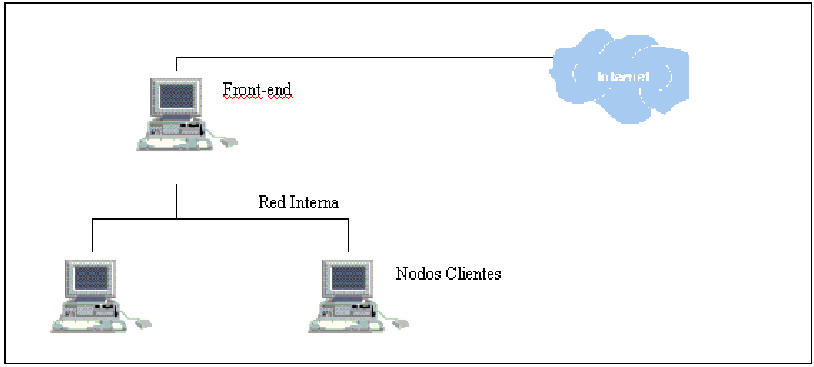
\epsfig{file=imagenes/intro/arquitectura.eps, width=4.25in}
\caption{Arquitectura gen�rica de un cluster Beowulf}
\end{center}
\end{figure}

La topolog�a de red recomendada es un Bus, debido a la facilidad para proporcionar escalabilidad a la
hora de agregar nuevos nodos al cluster. Protocolos como Ethernet, Fast Ethernet, GigaEthernet, 10/100 Mbps Switched Ethernet,
etc, son tecnolog�as apropiadas para ser utilizadas en Beowulf.

Beowulf utiliza como sistema operativo cualquier distribuci�n Linux. Adem�s usa bibliotecas de paso
de mensajes como PVM y MPI.
\newpage
Sin lugar a duda los cluster presenta una alternativa importante para varios problemas particulares, no
solo por su econom�a, sino tambi�n porque pueden ser dise�ados y ajustados para aplicaciones espec�ficas.

\subsection{Clasificaci�n.}
Para establecer las diferencias entre los distintos tipos de sistemas Beowulf se presenta la siguiente
clasificaci�n.
\begin{itemize}
\item Clase I. Son sistemas compuestos por m�quinas cuyos componentes cumplen con la prueba
de certificaci�n ``Computer Shopper'' lo que significa que sus elementos son de uso com�n, y pueden ser adquiridos
muy f�cilmente en cualquier tienda distribuidora. De esta manera, estos clusters no est�n dise�ados para ning�n
uso ni requerimientos en particular.
\item Clase II. Son sistemas compuestos por m�quinas cuyos componentes no pasan la prueba de
certificaci�n ``Computer Shopper'' lo que significa que sus componentes no son de uso com�n y por tanto no pueden
encontrarse con la misma facilidad que los componentes de sistemas de la clase anterior. De tal manera, pueden
estar dise�ados para alg�n uso o requerimiento en particular. Las m�quinas ubicadas en esta categor�a pueden
presentar un nivel de prestaciones superior a las de la clase I.
\end{itemize}

\clearemptydoublepage
\include{instalacion}
\clearemptydoublepage
\chapter{ARRANQUE SIN DISCO O DISKLESS.}
\minitoc
\section{Introducci�n.}

Uno de los cambios m�s destacables del uso de la computadoras en los �ltimos a�os ha sido la expansi�n
de la conectividad de red con TCP/IP desde la mesa del despacho a toda la organizaci�n. La infraestructura
necesaria para soportar el crecimiento de la red, encaminadores, puentes, conmutadores y concentradores, ha
crecido a una velocidad similar.

El personal t�cnico lucha por mantenerse con las demandas de conectividad y los cambios, movimientos y
reconfiguraciones de red frecuentes, que caracterizan el entorno actual. Estas circunstancias han generado una necesidad
de mecanismos  que permitan automatizar la configuraci�n de nodos y la distribuci�n del sistema operativo y
del software en la red. La forma m�s efectiva de conseguirlo es almacenar los par�metros de configuraci�n e
im�genes del software en una o m�s estaciones de \emph{arranque} de red. Al arrancar, los sistemas interact�an con
un servidor de arranque, recogen los par�metros de arranque y, opcionalmente, descargan el software apropiado.

\section{Requisitos del protocolo de arranque.}

Algunas computadoras s�lo necesitan unas cuentas variables de configuraci�n antes de arrancar. Otras,
puede que deban disponer de una lista detallada, m�s larga, de valores de par�metros. A veces, las estaciones de
trabajo, los host con Unix y otros sistemas operativos necesitan descargar completamente los sistemas operativos.
Otros sistemas, como los encaminadores, puentes, conmutadores o incluso los concentradores puede que necesiten
informaci�n de configuraci�n de arranque y descargar software.

La inicializaci�n debe ser robusta y flexible. Dependiendo del tama�o de la red, su topolog�a y requisitos
de disponibilidad, podr�a ser m�s conveniente centralizar la informaci�n de arranque en un �nico servidor, distribuirla
por la red en varios servidores o replicarla.

Cada computador conectado a una red TCP/IP debe conocer la siguiente informaci�n:
\begin{itemize}
\item Su direcci�n IP.
\item Su m�scara de red.
\item La direcci�n IP de un router.
\item La direcci�n IP de un servidor de nombres.
\end{itemize}
Esta informaci�n se guarda normalmente en ficheros de configuraci�n, a los que accede el SO en el
arranque.
	
�Qu� ocurre con los computadores sin disco?
	
Podr�a guardarse el S.O y el software de red en la ROM de la ethernet, pero esa informaci�n no es conocida
de antemano por el fabricante ya que define la red a la que se va a conectar el computador.

Disponemos de tres protocolos que nos permitir�n transferir esta informaci�n por la red:
\begin{itemize}
\item\textbf{RARP} (Reverse Address Resolution Protocol) s�lo proporciona la direcci�n IP al computador
sin disco. Debido a esto RARP no est� implementado en la mayor�a de los sistemas y se ha eliminado totalmente
de TCP/IP v6.
\item\textbf{BOOTP} (Bootstrap Protocol) es un protocolo cliente/servidor dise�ado para proporcionar los
cuatro tipos de informaci�n mencionados anteriormente, a un computador sin disco.
\item\textbf{DHCP} (Dinamic Host Configuration Protocol) es una extensi�n de BOOTP, es decir, lo mejora.
\end{itemize}

\section{Objetivos del arranque por red.}
\begin{itemize}
\item Reducir los costes de mantenimiento del software en gran cantidad de m�quinas. Con el
arranque por red los ficheros son mantenidos en un servidor central, esto conlleva a la ventaja de poder ser
actualizados en una sola m�quina.
\item La posibilidad de conmutar entre sistemas operativos sin tener que cargar el software cada
vez que se cambie de un sistema a otro.
\item Usar ordenadores en lugares donde los discos duros no son suficientemente resistentes, como
podr�a ser en la planta de una factor�a, en la que �stos pueden ser relativamente fr�giles.
\item Facilita el traspaso de equipos de una persona a otra. Por ejemplo, si en una empresa un
equipo pasa de una persona a otra, �sta no tendr� que hacer un traspaso de informaci�n sino que, como todo se
encuentra en el mismo servidor, bastar� con entrar con el nuevo usuario.
\item Reducir el coste econ�mico. El tener equipos sin disco duros reduce en gran medida el coste
de un equipo.
\end{itemize}
	
\section{Introducci�n DHCP.}

Las siglas DHCP significan Dinamic Host Configuration Protocol. Es utilizado para grandes redes. El
daemon act�a d�ndole informaci�n de la red a las estaciones de trabajo, tales como IP Address, Subnet Mask,
DNS Server, Gateway, etc.

DHCP ha sido creado por el Grupo de Trabajo Dynamic Host Configuration del IETF (Internet Engineering
Task Force, organizaci�n de voluntarios que define protocolos para su uso en Internet). Su definici�n se
encuentra en los RFC's 2131, el protocolo DHCP, y el 2132, opciones de DHCP.

Al igual que otros protocolos similares, utiliza el paradigma cliente-servidor, para que los nodos
clientes obtengan su configuraci�n del nodo servidor.
	
El protocolo de Configuraci�n Din�mica de Hosts (DHCP) permite la transmisi�n de la configuraci�n de
los hosts sobre una red TCP/IP. Este protocolo se encarga de la configuraci�n autom�tica de los par�metros de
red, utilizando direcciones.

DHCP es una extensi�n de BOOTP, es decir, mejora BOOTP, y es compatible con �l (un cliente puede realizar
una petici�n est�tica BOOTP a un servidor DHCP)

DHCP es un protocolo que permite asignar direcciones IP din�micas, de forma totalmente autom�tica. Por
ello no pierde las prestaciones de BOOTP, su predecesor, sino que las ampl�a permitiendo nuevas formas de
asignaci�n de direcciones y nuevas opciones para poder pasar a los clientes toda la informaci�n necesaria.
DHCP es un protocolo implementado en los principales sistemas operativos as� como otros dispositivos.

DHCP puede usarse cuando el n�mero de IPs es menor que el n�mero de computadores y todos no est�n
conectados a la vez, como en un proveedor de servicio de Internet (ISP).

DHCP est� formado por dos partes: un protocolo para el intercambio de los par�metros de red espec�ficos
de cada host y un mecanismo para la asignaci�n de direcciones de red.

Un servidor DHCP tiene dos bases de datos. La primera es est�tica, al igual que BOOTP y la segunda
contiene una pila de direcciones IP disponibles. Esta segunda base de datos hace a DHCP din�mico. Cuando un
cliente DHCP pide una direcci�n IP temporal, DHCP la coge de la pila de direcciones IP disponibles y se la
asigna durante un periodo de tiempo negociado.

El servidor admite tres tipos de configuraci�n de direcciones IP:
\begin{enumerate}
\item Est�tica. Se configura en el servidor la direcci�n de red que se corresponde con la
direcci�n LAN del cliente (equivalente a BOOTP).
\item Din�mica, por tiempo ilimitado. Se indica un rango de direcciones que se asignan a cada
cliente de car�cter permanente, hasta que el cliente la libera.
\item Din�mica, arrendada. Las direcciones se otorgan por un tiempo ilimitado. Un cliente
debe renovar su direcci�n para poder seguir utiliz�ndola.
\end{enumerate}

Cuando el servidor DHCP recibe una petici�n, primero chequea su base de datos est�tica. Si existe una
entrada para esa direcci�n f�sica, se devuelve la direcci�n IP est�tica correspondiente. Si no se encuentra
la entrada, el servidor selecciona una IP disponible de la base de datos din�mica y a�ade la nueva asociaci�n
a la base de datos.

\begin{itemize}\item\textbf{Alquiler}:
\begin{itemize}\item La direcci�n asignada desde la pila es temporal. El servidor DHCP emite un alquiler
por un periodo determinado de tiempo. Cuando el alquiler termina, el cliente debe, dejar de usar la IP o renovar
el alquiler. El servidor tiene la opci�n de aceptar o denegar la renovaci�n.
\end{itemize}\end{itemize}
\begin{itemize}\item\textbf{Operaci�n}:
El cliente realiza los siguientes pasos:
\begin{itemize}\item Env�a un mensaje \emph{DHCPDISCOVER} broadcast usando el puerto destino 67.
\item Aquellos servidores que puedan dar este tipo de servicio responden con un mensaje DHCPOFFER,
donde se ofrece una IP que ser� bloqueada. En estos mensajes tambi�n puede ofrecer la duraci�n del alquiler que
por defecto es de una hora. Si los clientes no reciben dicho mensaje, intenta establecer conexi�n cuatro veces
m�s, cada dos segundos, si a�n as� no hay respuesta, el cliente espera cinco minutos antes de intentarlo de nuevo.
\item El cliente elige una de las IPs ofertadas y env�a un mensaje DHCPREQUEST al servidor
seleccionado.
\item El servidor responde con un mensaje DHCPACK y crea la asociaci�n entre la direcci�n f�sica
del cliente y su IP. Ahora el cliente usa la IP hasta que el alquiler expire.
\item Antes de alcanzar el 50\% del tiempo del alquiler, el cliente env�a otro mensaje
DHCPREQUEST para renovar el alquiler.
\item Si el servidor responde con DHCPACK, el cliente puede seguir usando la IP durante otro
periodo de tiempo. Si se recibe un DHCPNACK, el cliente debe de dejar de usar esa IP y empezar de nuevo el
proceso de obtenci�n de una IP.
\item Si despu�s de transcurrir el 87.5\% del alquiler no se recibe respuesta, se manda otro
DHCPREQUEST. Si se recibe un DHCPACK antes de que expire el tiempo de alquiler, se obtiene m�s tiempo de
alquiler. En caso contrario, se debe comenzar de nuevo el proceso de obtenci�n de una IP. El cliente puede
terminar el alquiler antes de que expire el tiempo. En este caso, el cliente env�a un mensaje DHCPRELEASE al
servidor.

\begin{figure}[h!]
\begin{center}
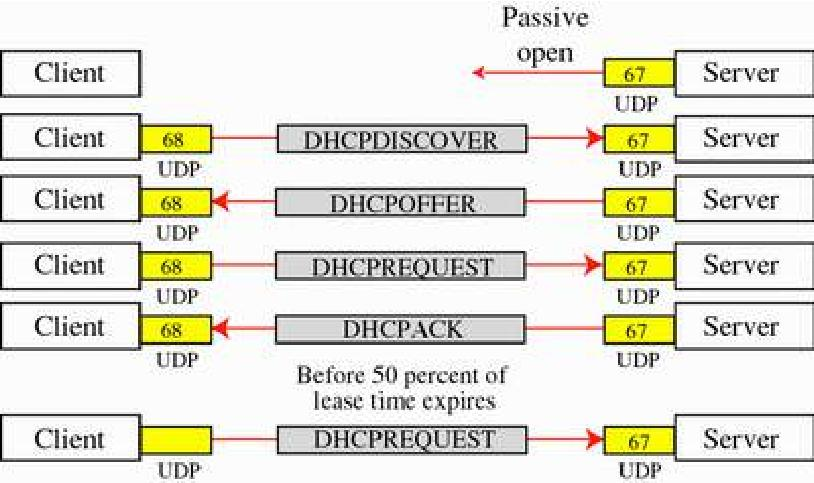
\epsfig{file=imagenes/dhcp/operaciondhcp.eps, width=3.25in}
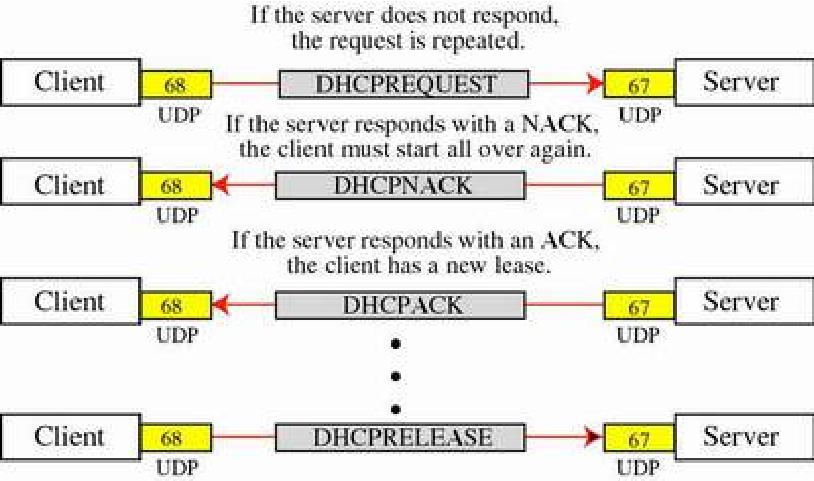
\epsfig{file=imagenes/dhcp/operaciondhcp1.eps, width=3.25in}
\caption{Funcionamiento DHCP}
\end{center}
\end{figure}
\end{itemize}\end{itemize}	

\begin{itemize}\item\textbf{Formato del paquete}:
	
Para hacer DHCP compatible con BOOTP, los dise�adores de DHCP han usado casi el mismo formato
de paquete. Solo se ha a�adido un bit de control al paquete. Sin embargo, se han a�adido opciones extra para
permitir las diferentes interacciones con el servidor. Los campos diferentes de DHCP son los siguientes:
\begin{itemize}
\item Flag: 1 bit. El primero del campo sin uso, que permite al cliente el forzar que
la respuesta del servidor sea broadcast en vez de unicast. Si la respuesta es unicast, la direcci�n destino
sera la del cliente y este no la conoce, por lo que puede descartar el mensaje. Al ser broadcast, todos los
computadores reciben y procesan el mensaje.

\begin{figure}[h!]
\begin{center}
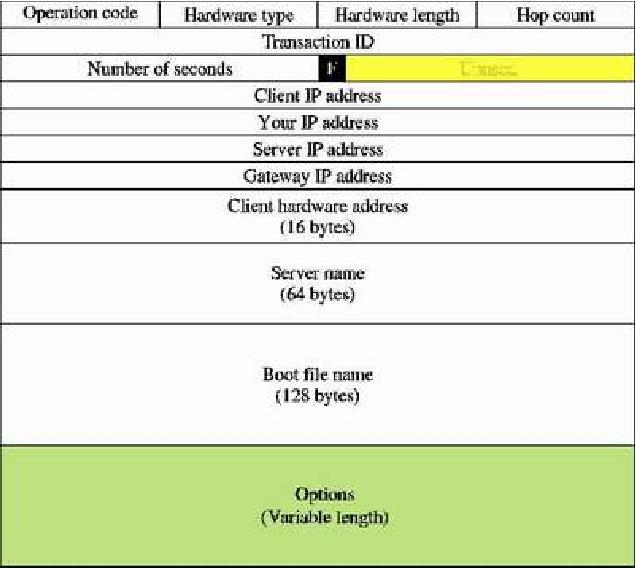
\epsfig{file=imagenes/dhcp/formatodhcp.eps, width=3.25in}
\caption{Formato opciones}
\end{center}
\end{figure}
\end{itemize}

\item\textbf{Opciones}: Se han a�adido varias posibiliades a la lista de opciones. La opci�n con
etiqueta 53 es la que define el tipo de interacci�n entre el cliente y el servidor. Otras opciones definen
par�metros con el tiempo de alquiler, etc. El campo de opci�n en DHCP puede tener hasta 312 bytes.
		
\begin{figure}[h!]
\begin{center}
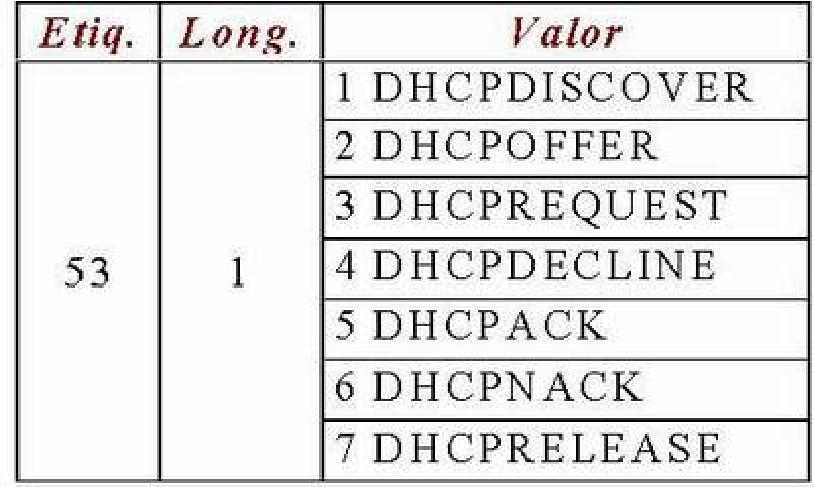
\epsfig{file=imagenes/dhcp/formatodhcp1.eps, width=3.25in}
\caption{Opciones}
\end{center}
\end{figure}
\end{itemize}
		
La asignaci�n de direcciones IP se configurar� de un modo u otro, dependiendo de cada situaci�n. Puede
interesar un direccionamiento est�tico para clientes sin disco o por facilidades administrativas, pero
controlando la asignaci�n de cada direcci�n a cada cliente (es mas c�modo para el administrador configurar
un servidor, que cada cliente; interesa el direccionamiento est�tico para evitar que se conecten clientes no
identificados o por otras razones, como la configuraci�n DNS).

El direccionamiento din�mico por tiempo ilimitado se utiliza cuando el n�mero de clientes no var�a
demasiado, facilitando mucho la tarea del administrador.

El arrendamiento de direcciones se emplea para racionar las direcciones IP, minimizando el coste
administrativo. En funci�n de la frecuencia de inserciones/eliminaciones de clientes y de la cantidad
de direcciones disponibles se conceder� un mayor o menor tiempo de arrendamiento. El tiempo sera bajo (ej.
15 minutos); si se conectan/desconectan los clientes con mucha frecuencia e interesa que este disponible
el m�ximo n�mero de direcciones. Por el contrario se utilizar� un tiempo largo para que cada cliente mantenga
su direcci�n IP (ej. en una universidad un tiempo de 4 meses, tiempo m�ximo que esta desconectado en vacaciones
para asumir que el cliente ya no esta en la red). Un port�til puede tener una direcci�n permanente o de larga
duraci�n en su red habitual de trabajo y tiempos cortos en otras redes.


\section{Caracter�sticas de DHCP.}

El protocolo de configuraci�n din�mico de host extiende significativamente las posibilidades de BOOTP.
Las mejoras mas importantes son:
        \begin{itemize}
		\item Administraci�n m�s sencilla.
		\item Configuraci�n automatizada.
		\item Permite cambios y traslados.
		\item Posibilidad de que el cliente solicite los valores de ciertos par�metros.
		\item Nuevos tipos de mensajes de DHCP que soportan interacciones cliente/servidor robustas.
	\end{itemize}

\section{�Qu� ventajas me da el DHCPd?}

El instalar un sistema DHCP en su red, le ahorra un trabajo de configuraci�n para su red. Todas las
computadoras piden informaci�n de la red y se configuran autom�ticamente, muy recomendable para un administraci�n
f�cil.

\section{Ejemplo te�rico del funcionamiento del arranque por red a trav�s del protocolo DHCP.}

Para que un ordenador, que act�a como cliente, pueda arrancar por red, el servidor deber� pasarle
la siguiente informaci�n:
\begin{itemize}
\item Informaci�n de red. Que podr�a estar formada por lo siguiente: direcci�n IP, servidor
de arranque y el fichero del que debe arrancar. Estos datos pueden varias dependiendo de las necesidades de cada
uno.
\item Un sistema de ficheros con el que trabajar.
\item La imagen (n�cleo del sistema operativo) para realizar el arranque.
\end{itemize}
	
Si tenemos una red formada por ordenadores sin disco (DC-Diskeless Computer) teniendo estos una ROM
para arrancar por red, se diferenciar�n unos de otros gracias a la direcci�n Ethernet.

Un ejemplo de intercambio ser�a el siguiente:
\begin{quote}
DC:Hola, mi direcci�n hardware es 00:60:08:C7:A3:D8, por favor, dame mi direcci�n IP.
		
Servidor DHCP: (busca la direcci�n en su base de datos) Tu nombre es host1, tu direcci�n
IP es 192.168.1.2, tu servidor es 192.168.1.1. En el caso que necesite un fichero del que se supone que debe
arrancar se alojar� en /tftpboot/.

La petici�n de DHCP se realiza en forma de broadcast dentro de la red local, de forma que cualquier
servidor de DHCP que pudiera responder a la petici�n, lo har�a.

Despu�s de obtener la direcci�n IP, el DC debe conseguir la imagen del sistema operativo y lanzarlo
a ejecuci�n. En esta fase, se usa otro protocolo TCP/IP, TFTP (Trivial File Transfer Protocol).�ste es una
versi�n reducida del FTP (File Transfer Protocol). El TFTP no contempla autentificaci�n, trabaja a trav�s
de UDP (User Datagram Protocol) en vez de TCP (Transmisi�n Control Protocol).

La implementaci�n de UDP en un ordenador de arranque sin disco puede ser suficientemente reducida como
para caber en una ROM. Existe la posibilidad de simular esta ROM a trav�s de un disquete. Debido a que UDP es un
protocolo orientado a la transmisi�n por bloques la transferencia se realiza bloque a bloque, de la siguiente forma:

DC: Dame el bloque 1 de /tftpboot/maquina1
	
TFTP servidor: Aqu� lo tienes
	
DC: Dame el bloque 2, y as� en adelante, hasta que se transfiere el fichero completo para almacenarlo
en RAM.
\end{quote}
El funcionamiento consiste, b�sicamente, en el reconocimiento de cada bloque, y la p�rdida de paquetes
se soluciona mediante su retransmisi�n al cabo de un tiempo establecido. Cuando todos los bloques han sido
recibidos, la ROM de arranque de la red pasa el control a la imagen del sistema operativo.

Finalmente, para poner en funcionamiento un sistema operativo, se le debe proporcionar un sistema de
ficheros ra�z. El protocolo utilizado por Linux y otros sistemas UNIX es normalmente NFS (Network File System),
 aunque no es el �nico.

En este caso el c�digo no necesita estar grabado en la ROM, sino que forma parte del sistema operativo
que acabamos de cargar. El sistema operativo debe ser capaz de ejecutarse con un sistema de ficheros ra�z NFS,
 en vez de un disco real.

\section{Preparaci�n de la m�quina servidora para atender peticiones por la red.}
\subsection{Creaci�n del sistema de ficheros para los PC clientes o nodos del cluster.}
	
Los directorios de cada uno de los posibles clientes de nuestro servidor se van a encontrar dentro del
directorio \textbf{/tftpboot}. La estructura de este directorio tendr� la siguiente forma:
\begin{quote}
\begin{em}
/tftpboot/nombre\_m�quina\_cliente1\newline
/tftpboot/nombre\_m�quina\_cliente2
\end{em}
\end{quote}
Dentro de los directorios clientes debemos crear la jerarqu�a de directorios necesaria para el sistema
de ficheros, es decir, tendr� la propia estructura del sistema de ficheros de Linux:
\begin{quote}
\begin{verbatim}
/tftpboot/nombre_m�quina_cliente/bin
/		"		  /dev
/		"		  /etc
/		"		  /lib
/		"		  /sbin
/		"		  /var
/		"		  /home
/		"		  /mnt
/		"		  /proc
/		"		  /root
/		"		  /tmp
/		"		  /usr
\end{verbatim}
\end{quote}
Para crear esta estructura interna a cada directorio cliente tenemos que ejecutar las siguientes �rdenes
de comandos en el front-end:
\begin{quote}
\begin{em}
\$$>$cd /tftpboot/nombre\_m�quina\_cliente\newline
\$$>$cp -r /bin .\newline
\$$>$cp -ra /dev .\newline	
\$$>$cp -ra /etc .\newline
\$$>$cp -r /lib .\newline	
\$$>$cp -r /sbin .\newline
\$$>$cp -r /var .\newline
\$$>$mkdir home\newline		
\$$>$mkdir mnt\newline			
\$$>$mkdir proc\newline		
\$$>$mkdir root\newline		
\$$>$mkdir tmp; tendr� permiso temporal $\Rightarrow$ chmod 0177\newline		
\$$>$mkdir usr
\end{em}
\end{quote}
Los directorios home, mnt, proc, root, tmp, es decir, los que solo creamos, ser�n montados desde el frontend
a trav�s del protocolo NFS, mientras que los directorios que copiamos son ``locales'' a cada uno de los clientes.
El proceso de montaje lo realiza el fichero \emph{/etc/fstab} local de cada cliente, que posteriormente ser�
explicado.
\subsection{Instalaci�n del dhcpd en el servidor.}
Para disponer del servidor DHCPD se tendr� que instalar el paquete \textbf{dhcpcd-1.3.18pl3-1.i386.rpm}
disponible en el CD-ROM de Red Hat Linux de la siguiente forma:
\begin{quote}
\emph{rpm -ivh dhcpcd-1.3.18pl3-1.i386.rpm}
\end{quote}
A continuaci�n se editar� el fichero \emph{/etc/rc.d/init.d/dhcpd}. En dicho fichero se tendr� que
indicar cual es el dispositivo de red para la red interna, para ello se tendr� que modificar la siguiente linea:
\begin{quote}
\emph{daemon /usr/sbin/dhcpd eth0}
\end{quote}
Sustituyendo eth0 por eth1 ya que es la ethernet para la red interna en nuestro caso concreto. Se guardar�
los cambios realizado a dicho fichero y se reiniciar� del daemon como se muestra a continuaci�n:
\begin{quote}
\emph{/etc/rc.d/init.d/dhcpd restart}	
\end{quote}
Una vez finalizada la tarea anterior, el siguiente paso a realizar ser� la activaci�n del servicio
 TFTP (Trivial File TransFer Protocol), debido que el posteriormente ser� utilizado por el paquete
Etherboot\footnote{Etherboot es un paquete software, cuya funci�n es la creaci�n de imagenes ROM que puede ser
descargables a trav�s de una red Ethernet para ser ejecutadas en computadores x86.} para transferir el n�cleo
por la red y otro ficheros necesario para el arranque sin disco. La ejecuci�n del demonio tftpd se realiza a
trav�s del superdemonio inetd. La configuraci�n de este superdemonio se encuentra en el archivo \emph{/etc/inted.conf}.
Este demonio es el encargado de arrancar autom�ticamente el servidor correspondiente a un servicio solicitado,
este servidor particular termina una vez que el servicio se ha proporcionado. Por lo tanto, el proceso inetd
est� a la escucha en los diferentes puertos correspondientes a los servicios disponibles.

El archivo \emph{/etc/inetd.conf} es utilizado por el proceso inetd cuando se lanza para conocer el
conjunto de puertos sobre los que se tiene que poner a la escucha. Este archivo contiene una l�nea por servicio,
cada l�nea suministra la siguiente informaci�n:
\begin{itemize}
\item El nombre del servicio.
\item El tipo de socket.
\item Una opci�n wait/nowait que se utiliza para las comunicaciones en modo no orientado a conexi�n
(dgram), las otras se utilizan siempre con la opci�n nowait. La opci�n wait evita, en el modo orientado a conexi�n,
la ejecuci�n de varios servidores a la escucha sobre un mismo puerto.
\item Un nombre de usuario que ser� propietario del proceso demonio asociado al servicio cuando se cree.
\item La referencia absoluta del archivo que contiene el programa que proporciona el servicio.
\item Una lista de par�metros para el programa.
\end{itemize}
	
Asi pues, se tendr� que activar la l�nea correspondiente al tftp eliminando la marca de comentario (\#)
para poder ejecutar el demonio tftpd:
\begin{quote}
\emph{tftp dgram udp wait root /usr/sbin/tcpd in.tftpd /tftpboot}
\end{quote}
El archivo \emph{/etc/services} contiene la lista de servicios de Internet conocidos. Un servicio se
caracteriza por su nombre, un n�mero de puerto, un protocolo y una lista de alias. El servicio anterior
describe un servicio est�ndar en Internet basados en el protocolo UDP.

Se deber� modificar el archivo \emph{etc/services} descomentando las siguientes dos l�neas:
\begin{quote}
\emph{tftp 69/udp \#TFTP server}
\end{quote}
Una vez que se han modificado los dos archivos anteriores debemos de reiniciar el superdemonio inetd
mediante la orden:
\begin{quote}
\emph{kill -HUP PID\_de\_inetd}
\end{quote}
	
\subsection{Configuraci�n del dhcpd en el servidor.}	

El demonio dhcpd tiene un archivo de configuraci�n llamado \emph{/etc/dhcpd.conf}. Finalizada la
realizaci�n de los pasos anteriores se proceder� a configurar las opciones DHCP creando o editando el fichero
anterior. Para este caso concreto dicho fichero presentar� la siguiente configuraci�n:
\begin{em}
\begin{quote}
\#red interna\newline
subnet 192.168.1.0 netmask 255.255.255.0 \{ \newline
option broadcast-address 192.168.1.255;
\begin{quote}
host pc1\{
\begin{quote}
hardware ethernet 00:50:04:09:DA:EB;\newline
fixed-address 192.168.1.2; \newline
option host-name "pc1";\newline
filename "/tftpboot/pc1/vmlinuz.nodos";
\end{quote}	
\}\newline
host pc2\{
\begin{quote}
hardware ethernet 00:50:DA:3D:2F:1C;\newline
fixed-address 192.168.1.3;\newline
option host-name "pc2";\newline
filename "/tftpboot/pc2/vmlinuz.nodos";
\end{quote}	
\}
\end{quote}
\end{quote}
\end{em}
A continuaci�n se realiza una aclaraci�n de la configuraci�n anterior:
\begin{quote}
\textbf{subnet 192.168.1.0 netmask 255.255.255.0}: Declaraci�n de la subred interna.\newline
\textbf{option broadcast-address}: Direcci�n de broadcast.\newline
\textbf{hosts pc1 }: Indica que la configuraci�n corresponde a la m�quina cliente pc1.\newline
\textbf{hardware ethernet}: Especifica el tipo de hardware y la direcci�n de la tarjeta de red de
la m�quina cliente.\newline
\textbf{fixed-address}: Direcci�n IP que se asigna a la m�quina cliente con la direcci�n de red arriba
indicada.\newline
\textbf{option host-name "pc1.cluster.psa.es"}: Indica el nombre que se le asigna a la m�quina cliente.
\end{quote}
Terminada la configuraci�n del servidor DHCP se reiniciar�a el demonio DHCP como anteriormente se ha
comentado.

\subsection{Configuraci�n del fichero /etc/hosts.}	
	
	Este fichero contiene las informaciones relativas a las diferentes m�quinas de la red local a la que
pertenece el sistema. Contiene la tabla de correspondencias entre la direcci�n Internet y un nombre simb�lico.
Dentro de una red este nombre simb�lico contiene una componente �nica. A cada m�quina de la red le corresponde
una l�nea de dicho archivo quedando la siguiente tabla:
\begin{quote}
\begin{em}
127.0.0.1	localhost.localdomain	localhost\newline
192.168.1.1 	pc0.cluster.psa.es	pc0\newline
192.168.1.2	pc1.cluster.psa.es	pc1\newline
192.168.1.3	pc2.cluster.psa.es	pc2
\end{em}
\end{quote}

\subsection{Configuraci�n del fichero /etc/exports.}

Este archivo sirve como la lista de control de acceso para sistemas de ficheros que pueden ser exportados
a clientes NFS. Cada l�nea contiene un punto de montaje y una lista de m�quinas o nombres de grupo de red a las
que se les permite montar el sistema de ficheros en ese punto. Su estructura se muestra a continuaci�n:
\begin{quote}
\begin{em}
/tftpboot	*.cluster.psa.es(rw,no\_root\_squash)\newline
/bin		*.cluster.psa.es(rw,no\_root\_squash)\newline
/usr		*.cluster.psa.es(rw,no\_root\_squash)\newline
/sbin		*.cluster.psa.es(rw,no\_root\_squash)\newline
/home		*.cluster.psa.es(rw,no\_root\_squash)\newline
/lib		*.cluster.psa.es(rw,no\_root\_squash)\newline
/boot		*.cluster.psa.es(rw,no\_root\_squash)\newline
/root		*.cluster.psa.es(rw,no\_root\_squash)\newline
/etc/passwd	*.cluster.psa.es(rw,no\_root\_squash)\newline
/etc/group	*.cluster.psa.es(rw,no\_root\_squash)
\end{em}
\end{quote}
	
donde:
\begin{quote}
\textbf{rw}: Permitir pedidos de lectura/escritura.\newline
\textbf{no\_root\_squash}: Deshabilita la opci�n de root squashing, permitiendo conexi�n en modo root. Esta
opci�n es particularmente �til para clientes sin disco.
\end{quote}

\subsection{Preparaci�n de la configuraci�n del cliente.}
Como ya se ha creado una estructura de directorios donde alojar el sistema de ficheros de las m�quinas
clientes en los apartados anteriores, y se han copiado los directorios que contienen la configuraci�n de Linux
de la m�quina servidora, ahora se tiene que adaptar para cada m�quina los ficheros de configuraci�n.\newline
\textbf{Nota:} Todos los cambios que se van a realizar a continuaci�n se har�n sobre los archivos de configuraci�n
que est�n en la ruta \emph{/tftpboot/pc1}, es decir que cuando se diga que se modifica el \emph{etc/hosts} se
esta haciendo referencia al archivo que existe en la ruta \emph{/tftpboot/pc1/etc/hosts}.

\subsection{Configuraci�n del ficheros /etc/HOSTNAME.}
No se dar� ningun nombres, es decir, se deber� dejar el archivo vac�o.
	
\subsection{Configuraci�n del fichero /etc/hosts.}
En este constar� unicamente las direcciones IP de los clientes que van a formar la red interna:
\begin{quote}
\begin{em}
127.0.0.1	localhost.localdomain	localhost\newline
192.168.1.1 	pc0.cluster.psa.es	pc0\newline
192.168.1.2	pc1.cluster.psa.es	pc1\newline
192.168.1.3	pc2.cluster.psa.es	pc2
\end{em}
\end{quote}

\subsection{Configuraci�n del fichero /etc/fstab.}
Este archivo contiene la tabla del sistema de ficheros utilizado por el cliente pc1. Hay que indicar
los directorios que se van a montar v�a NFS. El contenido debe quedar de la siguiente forma:
\begin{quote}
\begin{em}
pc0:/tftpboot/pc1 /	nfs	defaults	1	1\newline
pc0:/bin		/bin	nfs	defaults	1	1\newline
pc0:/usr		/usr	nfs	defaults	1	1\newline
pc0:/sbin		/sbin	nfs	defaults	1	1\newline
pc0:/home		/home	nfs	defaults	1	1\newline
pc0:/lib		/lib	nfs	defaults	1	1\newline
pc0:/boot		/boot	nfs	defaults	1	1\newline
none              /proc     proc    defaults        0 0\newline
none              /dev/pts  devpts  gid=5,mode=620  0 0
\end{em}
\end{quote}
As� pues el directorio ra�z de la m�quina pc1 va a ser el directorio /tftpboot/pc1 de la m�quina pc0
siendo este el servidor o front-end.

\subsection{Configuraci�n del fichero /etc/sysconfig/network.}
Este archivo presenta informaci�n de red relativa a la m�quina necesaria para la red, para nuestro
caso del cliente pc1 queda de la siguiente forma:
\begin{quote}
\begin{em}
NETWORKING=yes\newline
HOSTNAME=\newline
FORWARD\_IP=no
\end{em}
\end{quote}

\subsection{Configuraci�n del fichero /etc/sysconfig/network-scripts/ifcfg-eth0.}
Este archivo especifica el nombre del dispositivo de la interfaz de red, la direcci�n IP, la m�scara
de red, la direcci�n de red, la direcci�n de broadcast e informaci�n sobre el modo de arranque. Los datos para
la m�quina pc1 son los siguientes:
\begin{quote}
\begin{em}
DEVICE="eth0"\newline
BOOTPROTO="dhcp"\newline
BROADCAST=\newline
IPADDR=\newline
NETMASK=\newline
NETWORK=\newline
ONBOOT="yes"
\end{em}	
\end{quote}
En este momento la m�quina cliente quedar�a bien configurada para que hiciese el arranque, lo que pasa
es que cuando el proceso de arranque intenta chequear los discos duros, el sistema se queda bloqueado ya que
esta trabajando NFS. Para solucionar este problema se presenta el siguiente apartado.

\subsection{Configuraci�n del fichero /etc/rc.d/rc.sysinit.}
En este archivo tenemos que comentar o eliminar las l�neas que hacen referencia al chequeo de las
unidades. Estas l�neas son las siguientes:
\begin{quote}
\begin{em}
if [ -f /fsckoptions ]; then
\begin{quote}fsckoptions=`cat /fsckoptions'\end{quote}
else                 f
\begin{quote}fsckoptions=\end{quote}
fi\newline
if [ -f /forcefsck ]; then
\begin{quote}fsckoptions=``-f \$fsckoptions''\end{quote}
fi\newline
if [ ``\$BOOTUP'' != ``serial'' ]; then
\begin{quote}fsckoptions='' -C \$fsckoptions"\end{quote}
else
\begin{quote}fsckoptions=`` -V \$fsckoptions''\end{quote}
fi\newline
\_RUN\_QUOTACHECK=0\newline
if [ ! -f /fastboot ]; then
\begin{quote}
STRING=``Checking root filesystem''\newline
echo \$STRING\newline
initlog -c ``fsck -T -a \$fsckoptions /''\newline
rc=\$?
\end{quote}
if [ "\$rc" = "0" ]; then
\begin{quote}
success "\$STRING"
echo
\end{quote}
elif [ "\$rc" = "1" ]; then
\begin{quote}
passed "\$STRING"
echo
\end{quote}
fi\newline
\# A return of 2 or higher means there were serious problems.\newline
if [ \$rc -gt 1 ]; then
\begin{quote}
failure "\$STRING"\newline
echo\newline
echo\newline
echo "*** An error occurred during the file system check."\newline
echo "*** Dropping you to a shell; the system will reboot"\newline
echo "*** when you leave the shell."\newline
PS1=``(Repair filesystem) \# \# ''; export PS1\newline
sulogin\newline
echo ``Unmounting file systems''\newline
umount -a\newline
mount -n -o remount,ro /\newline
echo ``Automatic reboot in progress.''\newline
reboot -f\newline
elif [ ``\$rc'' = ``1'' ]; then\newline
\begin{quote}\_RUN\_QUOTACHECK=1\end{quote}
fi
\end{quote}
fi\newline
\_RUN\_QUOTACHECK=0\newline
\# Check filesystems\newline
if [ ! -f /fastboot ]; then\newline
STRING="Checking filesystems"\newline
echo \$STRING\newline
initlog -c ``fsck -T -R -A -a \$fsckoptions''\newline
rc=\$?\newline
if [ "\$rc" = "0" ]; then
\begin{quote}
success "\$STRING"\newline
echo
\end{quote}
elif [ "\$rc" = "1" ]; then
\begin{quote}
passed "\$STRING"\newline
echo
\end{quote}
fi\newline
\# A return of 2 or higher means there were serious problems.\newline
if [ \$rc -gt 1 ]; then
\begin{quote}
failure "\$STRING"\newline
echo\newline
echo\newline
echo ``*** An error occurred during the file system check.''\newline
echo ``*** Dropping you to a shell; the system will reboot''\newline
echo ``*** when you leave the shell."\newline
PS1=``(Repair filesystem) \# \# ''; export PS1\newline
sulogin\newline
echo ``Unmounting file systems''\newline
umount -a\newline
mount -n -o remount,ro /\newline
echo ``Automatic reboot in progress.''\newline
reboot -f\newline
elif [ ``\$rc'' = ``1'' -a -x /sbin/quotacheck ]; then\newline
\_RUN\_QUOTACHECK=1
\end{quote}
fi\newline
fi
\end{em}	
\end{quote}

\subsection{Comprobaci�n del arranque v�a NFS.}
Una vez acabada la configuraci�n de los clientes debemos comprobar que podemos montar la estructura de
directorios creada para los clientes v�a NFS realizando los siguientes pasos:

Exportar los directorios:
\begin{quote}
\emph{exportfs -av}
\end{quote}

Montar los directorios en el cliente:
\begin{quote}
\emph{mount -t nfs nb\_servidor:/tftpboot/directorio\_cliente /directorio\_destino}
\end{quote}

En este caso quedar�a:
\begin{quote}
\emph{mount -t nfs pc0:/tftpboot/pc1 /mnt}
\end{quote}

Si no lo monta correctamente se revisar� todos los pasos realizados.

\section{Configuraci�n del n�cleo.}\label{sec:OK}

El usuario root es el �nico que tiene permisos para poder compilar el kernel.
	
A continuaci�n se va ha indicar los m�dulos que debe tener el kernel para poder realizar la petici�n de
direcci�n IP y poder montar su sistema de ficheros a trav�s de la red. La opciones que se tendr� que activar son:
\begin{itemize}
\item En el apartado LOADABLE MODULE SUPPORT.
\begin{quote}
\emph{Enable loadable module support: Desactivado}		
\end{quote}
\item En el apartado NETWORKING OPTIONS.
\begin{quote}
\emph{IP kernel level autoconfiguration: Activado}\newline
\emph{BOOTP support: Activado}\newline
\emph{RARP support: Activado}\								
\end{quote}
\item En el apartado NETWORK FILE SYSTEM.
\begin{quote}
\begin{em}
NFS Filesystem support: Activado\newline
Root Filesystem on NFS: Activado\newline
NFS server support: Desactivado						
\end{em}
\end{quote}
\end{itemize}
	
Para poder compilar el kernel con las opciones anteriormente indicadas vamos a utilizar una herramienta
que nos mostrar� un men� en TCL/TK:
\begin{quote}
\emph{\$$>$cd /usr/src/linux}\newline		
\emph{\$$>$make xconfig}
\end{quote}
Una vez ejecutada esta herramienta se realizar� los pasos que muestran las siguientes figuras:

\begin{figure}[h!]
\begin{center}
\epsfig{file=imagenes/nucleo_diskeles/2.eps, width=3.25in}
\caption{Paso 1. Cargar preconfiguraci�n del n�cleo}
\end{center}
\end{figure}

\clearpage
\begin{figure}[h!]
\begin{center}

\epsfig{file=imagenes/nucleo_diskeles/1.eps, width=3.75in}
\caption{Paso 2. Cargar fichero}
\end{center}
\end{figure}

\begin{figure}[h!]
\begin{center}
\epsfig{file=imagenes/nucleo_diskeles/3.eps, width=3.75in}
\caption{Paso 3. Loadable module support}
\end{center}
\end{figure}

\clearpage	
\begin{figure}[h!]
\begin{center}
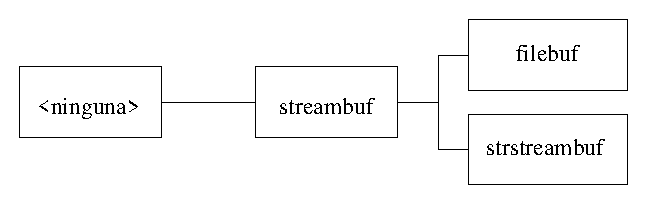
\epsfig{file=imagenes/nucleo_diskeles/4.eps, width=3.25in}
\caption{Paso 4. Desactivar loadable module support}
\end{center}
\end{figure}

\begin{figure}[h!]
\begin{center}
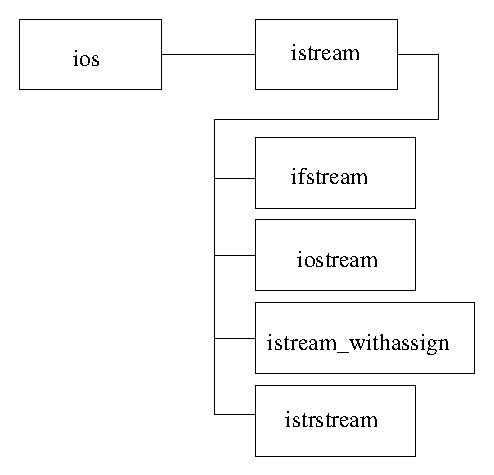
\epsfig{file=imagenes/nucleo_diskeles/5.eps, width=3.25in}
\caption{Paso 5. Networkin options}
\end{center}
\end{figure}


\begin{figure}[h!]
\begin{center}
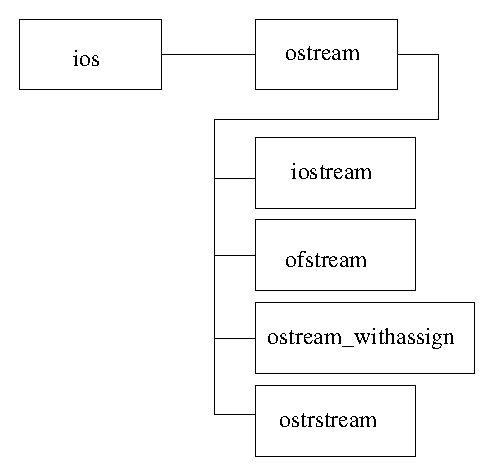
\epsfig{file=imagenes/nucleo_diskeles/6.eps, width=3.25in}
\caption{Paso 6. Activaci�n del protocolo BOOTP}
\end{center}
\end{figure}

\clearpage
\begin{figure}[h!]
\begin{center}
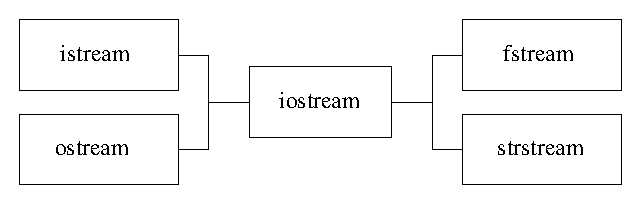
\epsfig{file=imagenes/nucleo_diskeles/7.eps, width=3.25in}
\caption{Paso 7. Networking File System}
\end{center}
\end{figure}

\begin{figure}[h!]
\begin{center}
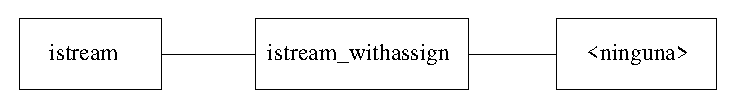
\epsfig{file=imagenes/nucleo_diskeles/8.eps, width=3.25in}
\caption{Paso 8. Activar NFS}
\end{center}
\end{figure}

\begin{figure}[h!]
\begin{center}
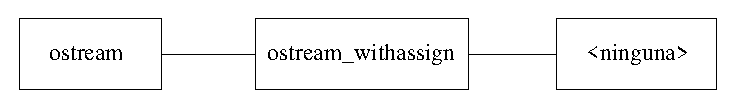
\epsfig{file=imagenes/nucleo_diskeles/9.eps, width=3.25in}
\caption{Paso 9. Guardar configuraci�n}
\end{center}
\end{figure}

\clearpage	
\begin{figure}[h!]
\begin{center}
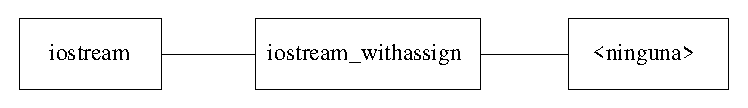
\epsfig{file=imagenes/nucleo_diskeles/10.eps, width=3.25in}
\caption{Paso 10. Guardar configuraci�n a un archivo}
\end{center}
\end{figure}

\begin{figure}[h!]
\begin{center}
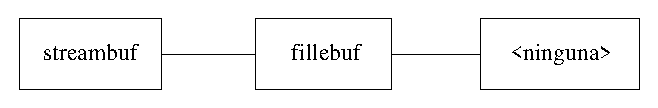
\epsfig{file=imagenes/nucleo_diskeles/11.eps, width=3.25in}
\caption{Paso 11. Salir}
\end{center}
\end{figure}

\begin{figure}[h!]
\begin{center}
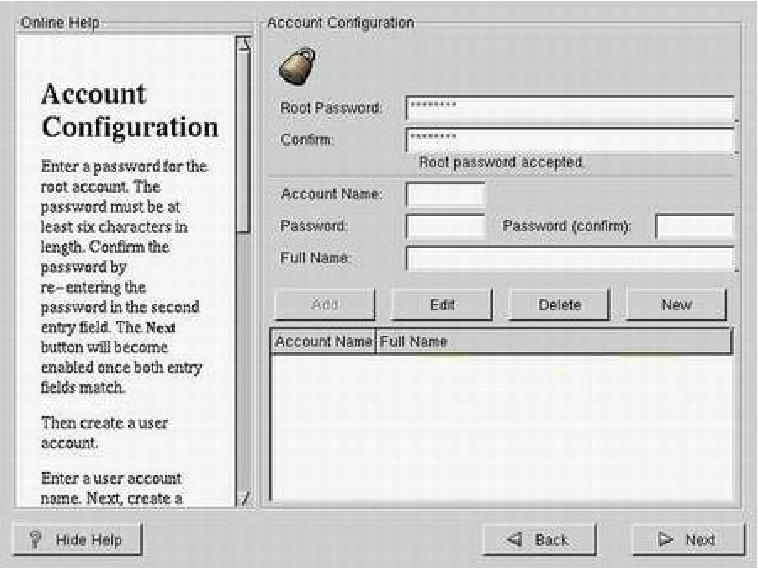
\epsfig{file=imagenes/nucleo_diskeles/12.eps, width=3.25in}
\caption{Paso 12. Configuraci�n finalizada}
\end{center}
\end{figure}

\section{Etherboot.}
\subsection{Introducci�n}
Etherboot es un paquete software, cuya funci�n es la creaci�n de imagenes ROM que puede ser
descargables a trav�s de una red Ethernet para ser ejecutadas en computadores x86.
Algunos adaptadores de red tienen un enchufe donde puede ser instalado o conectado un chip ROM.
Etherboot es c�digo que puede ser grabado en una ROM. Etherboot es usado normalmente para realizar
arranque sin disco o diskeless. Esto es beneficioso en varias situaciones, por ejemplo:
\begin{itemize}
\item Un X-Terminal.
\item Cluster de computadoras.
\item Routers.
\item Varias clases de servidores remotos, por ejemplo, un servidor de cinta que solo puede ser
accedido a trav�s del protocolo RMT.
\item Maquinas trabajando en entornos desfavorables para los discos duros.
\item Plataformas de usuario donde las particiones remotas son montadas a trav�s de la red y
se obtiene bajas velocidades en comparaci�n con los discos.
\item Mantenimiento software para cluster de igual configuraci�n a la estaci�n de trabajo central.
\end{itemize}
		
Etherboot inicia computadores mas r�pidamente que un disquete ya que no hay retardos en los giros
del disco, etc. Realizando un peque�o calculo se observar� que con una Ethernet de 10Mbit/s se enviar�
un kenel de 500kB en un par de segundos. Con una Ethernet de 100Mbit se obtendr� mejores resultados a�n.

En comparaci�n con el arranque desde dispositivos como puede ser un disco Flash, Etherboot posee
la ventaja de la administraci�n del software centralizado.

Etherboot trabaja con discos RAM, sistemas de ficheros NFS, o discos locales. Es un componente
tecnologico que puede ser combinado con otras tecnolog�as para actuar como deseamos.

Etherboot se utiliza generalmente para cargar Linux, FreeBSD o el DOS. No obstante los
formatos del fichero del protocolo y del cargador del programa inicial son generales.

Etherboot es Open Source bajo la GNU GPL2 (General Public Licence Version 2).
	
Los componentes necesitados por Etherboot son:
\begin{itemize}
\item Un cargador de carga inicial, usualmente una EEPROM de una tarjeta de red o instalado
en la flash BIOS.
\item Un servidor DHCP o BOOTP, que asigne una direcci�n IP cuando reciba una direcci�n MAC.
\item Un servidor TFTP, encargado de transmitir la imagen del kernel y otros ficheros requeridos
durante el proceso de arranque.
\end{itemize}
	
\subsection{Funcionamiento.}
A continuaci�n se describir� el funcionamiento del software Etherboot.
\begin{itemize}
\item Busca un servidor DHCP que en funci�n de su direcci�n MAC le asignar� una direcci�n IP.
\item Una vez asignada la direcci�n IP, solicitar� la transmisi�n del archivo con la imagen del n�cleo. Esta
transmisi�n la realizar� el TFTP.
\item Recibido el archivo con la imagen del n�cleo, ser� el n�cleo el encargado de seguir con el proceso de
arranque, es decir, solicitar� una IP a trav�s de DHCP y un servidor se le asignar� en funci�n de su direcci�n
MAC y solicitar� la transmisi�n del sistema archivos v�a NFS.
\end{itemize}

\subsection{Instalaci�n.}
Los fuentes del paquete Etherboot esta disponible en la web \url{http://etherboot.sourceforge.net/distribution.html}.
	
Una vez descargados dichos fuentes deber� ser compilados, a continuaci�n se muestran los pasos a
seguir para la instalaci�n de Etherboot:
\begin{enumerate}
\item Descargar de la web los paquetes etherboot-5.0.2.tar.gz y mknbi-1.2.tar.gz.
\item Descomprimir los paquetes utilizando tar xvfz nombre\_paquete.
\item Recompilar el n�cleo con las opciones seguidas en el punto \ref{sec:OK}, con los siguientes comandos:
\begin{quote}
\emph{\$$>$make dep;make clean;make bzImage}
\end{quote}
\item Copiar la imagen del n�cleo generada al directorio donde se haya descomprimido el paquete
mknbi-1.2.tar.gz. La imagen del n�cleo se encuentra en el directorio \emph{/usr/src/linux/arch\newline/i386/boot}
\item En el arranque no se puede usar el fichero \emph{bzImage}, generada en la compilaci�n del
n�cleo. Esta imagen debe ser convertida en una \emph{tagged image} (imagen etiquetada). Esta es una imagen normal
con una cabecera especial que le dice al cargador de arranque en red d�nde han de almacenarse los bytes en memoria
y en qu� direcci�n empieza el programa. Para crear esta imagen se usa el programa llamado \emph{mknbi-linux},
que nos prove� el paquete mknbi-1.2.tar.gz.

Posicionarse en el directorio donde se hay descomprimido el paquete mknbi-1.2.tar.gz (por
ejemplo \emph{/home/usuario/mknbi-1.2}), transformar la imagen del n�cleo, es decir, hacer una tagged imagen con
el siguiente comando:
\begin{quote}
\emph{./mknbi -format=elf -target=linux bzImage -output=vmlinuz.nodos}
\end{quote}
\item Copiar el archivo generado vmlinuz.nodos al directorio /tftpboot
\item Posicionarse sobre el directorio src dentro del directorio en el cual se haya descomprimido
el paquete etherboot-5.0.2.tar.gz, como por ejemplo \emph{/home/usuario/etherboot-5.0.2/src}	
\item Introducci�n de un disquete en la unidad de disco y escribir los siguiente comandos:
\begin{quote}
\emph{\$$>$make}\newline
\emph{\$$>$make bin/boot1a.bin $\Rightarrow$ se genera la imagen de los drivers de la
tarjeta de red} \newline
\emph{\$$>$make bin32/3c90x.rom $\Rightarrow$ esta l�nea variar� en funci�n de la tarjeta
de red, en este caso concreto una 3COM 3c905}\newline
\emph{\$$>$cat bin/boot1a.bin bin32/3c90x.rom $>$ /dev/fd0}\newline
\end{quote}
\end{enumerate}
	
Una vez finalizados los pasos anteriores ya estar�a preparado el disquete de arranque, solamente
quedar�a irse a un cliente y comprobar que el proceso de arranque v�a nfs funciona correctamente.
				
Los servicios m�nimos que deben estar corriendo en el cliente una vez que ha arrancado correctamente
son: \emph{identd, inet,netfs, network, portmap}. Si eliminamos algunos de estos servicios el cliente no funcionar�
correctamente.
	

\clearemptydoublepage
\chapter{Cortafuegos: Conceptos te\'oricos}
\section{Introducci\'on}
Seg\'un \cite{kn:firefaq}, un {\it firewall} o cortafuegos es un sistema o 
grupo de sistemas que hace cumplir una pol\'{\i}tica de control de acceso
entre dos redes. De una forma m\'as clara, podemos definir un cortafuegos como 
cualquier sistema (desde un simple {\it router} hasta varias redes en serie) 
utilizado para separar -- en cuanto a seguridad se refiere --
una m\'aquina o subred del resto, protegi\'endola as\'{\i} de servicios y 
protocolos que desde el exterior puedan suponer una amenaza a la seguridad. El
espacio protegido, denominado {\bf per\'{\i}metro de seguridad}, suele ser 
propiedad de la misma organizaci\'on, y la protecci\'on se realiza contra una 
red externa, no confiable, llamada {\bf zona de riesgo}.\\
\\Evidentemente la forma de aislamiento m\'as efectiva para cualquier 
pol\'{\i}tica de seguridad consiste en el aislamiento f\'{\i}sico, es decir, no
tener conectada la m\'aquina o la subred a otros equipos o a Internet (figura
\ref{lanwan} (a)). Sin embargo, en la mayor\'{\i}a de organizaciones --
especialmente en las de I+D -- los usuarios
necesitan compartir informaci\'on con otras personas situadas en muchas 
ocasiones a miles de kil\'ometros de distancia, con lo que no es posible un 
aislamiento total. El punto opuesto consistir\'{\i}a en una conectividad 
completa con la red (figura \ref{lanwan} (b)), lo que desde el punto de vista 
de la seguridad es muy
problem\'atico: cualquiera, desde cualquier parte del mundo, puede 
potencialmente tener acceso a nuestros recursos. Un t\'ermino medio entre ambas 
aproximaciones consiste en implementar cierta separaci\'on l\'ogica mediante un 
cortafuegos (figura \ref{lanwan} (c)).\\
\begin{figure}
\begin{center}
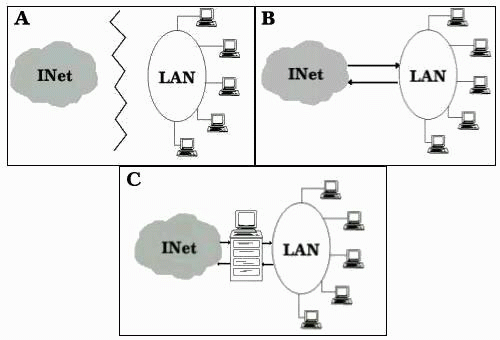
\includegraphics[width=\textwidth]{fw.png}
\caption{(a) Aislamiento. (b) Conexi\'on total. (c) {\it Firewall} entre la
zona de riesgo y el per\'{\i}metro de seguridad.}
\label{lanwan}
\end{center}
\end{figure}
\\Antes de hablar de cortafuegos es casi obligatorio dar una serie
de definiciones de partes o caracter\'{\i}sticas de funcionamiento de un {\it
firewall}; por m\'aquina o {\it host} {\bf basti\'on} (tambi\'en se denominan
{\bf gates}) se conoce a un sistema especialmente asegurado, pero en principio
vulnerable a todo tipo de ataques por estar abierto
a Internet, que tiene como funci\'on ser el punto de contacto de los usuarios
de la red interna de una organizaci\'on con otro tipo de redes. El {\it host}
basti\'on filtra tr\'afico de entrada y salida, y tambi\'en esconde la 
configuraci\'on de la red hacia fuera.\\
\\Por {\bf filtrado de paquetes} entendemos la acci\'on de denegar o permitir
el flujo de tramas entre dos redes (por ejemplo la interna, protegida con el
{\it firewall}, y el resto de Internet) de acuerdo a unas normas predefinidas;
aunque el filtro m\'as elemental puede ser un simple {\it router}, trabajando 
en el nivel de red del protocolo OSI, esta actividad puede realizarse 
adem\'as en un puente o en una m\'aquina individual. El filtrado tambi\'en se 
conoce como {\it screening}, y a los dispositivos que lo implementan se les
denomina {\bf chokes}; el {\it choke} puede ser la m\'aquina basti\'on o un
elemento diferente.\\
\\Un {\bf proxy} es un programa (trabajando en el nivel de aplicaci\'on de OSI)
que permite o niega el acceso a una aplicaci\'on determinada entre dos redes. 
Los clientes {\it proxy} se comunican s\'olo con los servidores {\it proxy}, 
que autorizan las peticiones y las env\'{\i}an a los servidores reales, o las
deniegan y las devuelven a quien las solicit\'o.\\
\\F\'{\i}sicamente, en casi todos los cortafuegos existen al menos un {\it 
choke} y una m\'aquina basti\'on, aunque tambi\'en se considera {\it firewall} 
a un simple {\it router} filtrando paquetes, es decir, actuando como {\it 
choke}; desde el punto de vista l\'ogico, en el cortafuegos suelen existir 
servidores {\it proxy} para las aplicaciones que han de atravesar el sistema, y
que se situan habitualmente en el {\it host} basti\'on. Tambi\'en se implementa
en el {\it choke} un mecanismo de filtrado de paquetes, y en alguno de los
dos elementos se suele situar otro mecanismo para poder monitorizar y detectar 
la actividad sospechosa.\\
\\En este cap\'{\i}tulo hablaremos de los tipos de cortafuegos m\'as 
habituales y de sus caracter\'{\i}sticas, as\'{\i} como de las posibles 
pol\'{\i}ticas de seguridad que pueden implementar; en el siguiente 
comentaremos aspectos de algunos de los cortafuegos m\'as utilizados hoy en 
d\'{\i}a, como {\it FireWall-1} o Cisco PIX Firewall. Los {\it firewalls} son 
cada vez m\'as
necesarios en nuestras redes, pero todos los expertos recomiendan que no se usen
{\bf en lugar de} otras herramientas, sino {\bf junto a} ellas; cualquier 
cortafuegos, desde el m\'as simple al m\'as avanzado, presenta dos 
grav\'{\i}simos problemas de seguridad: por un lado, centralizan todas las 
medidas en un \'unico sistema, de forma que si \'este se ve comprometido y 
el resto de nuestra red no est\'a lo suficientemente protegido el atacante 
consigue amenazar a toda la subred simplemente poniendo en jaque a una 
m\'aquina. El segundo problema, relacionado con \'este, es la falsa sensaci\'on
de seguridad que un cortafuegos proporciona: generalmente un administrador que
no disponga de un {\it firewall} va a preocuparse de la integridad de todas y
cada una de sus m\'aquinas, pero en el momento en que instala el cortafuegos
y lo configura asume que toda su red es segura, por lo que se suele descuidar
enormemente la seguridad de los equipos de la red interna. Esto, como acabamos
de comentar, es un grave error, ya que en el momento que un pirata acceda a
nuestro cortafuegos -- recordemos que es un sistema muy expuesto a ataques
externos -- autom\'aticamente va a tener la posibilidad de controlar toda 
nuestra red.\\
\\Adem\'as -- esto ya no es un problema de los {\it firewalls} sino
algo de sentido com\'un --, un cortafuegos evidentemente no protege contra 
ataques que no pasan por \'el: esto incluye todo tipo de ataques internos dentro
del per\'{\i}metro de seguridad, pero tambi\'en otros factores que {\it a
priori} no deber\'{\i}an suponer un problema. El t\'{\i}pico ejemplo de estos
\'ultimos son los usuarios que instalan sin permiso, sin conocimiento del 
administrador de la red, y muchas veces sin pensar en sus consecuencias, un
simple {\it modem} en sus PCs o estaciones de trabajo; esto, tan habitual en
muchas organizaciones, supone la violaci\'on y la ruptura total del 
per\'{\i}metro de seguridad, ya que posibilita accesos a la red no controlados
por el cortafuegos. Otro problema de sentido com\'un es la reconfiguraci\'on
de los sistemas al pasarlos de una zona a otra con diferente nivel de seguridad,
por ejemplo al mover un equipo que se encuentra en el \'area protegida a la
DMZ (veremos m\'as adelante lo que estas siglas significan); este acto -- que
en ocasiones no implica ni tan siquiera el movimiento f\'{\i}sico del equipo, 
sino simplemente conectarlo en una toma de red diferente -- puede ocasionar
graves problemas de seguridad en nuestra organizaci\'on, por lo que cada vez que
un cambio de este estilo se produzca no s\'olo es necesaria la reconfiguraci\'on
del sistema, sino la revisi\'on de todas las pol\'{\i}ticas de seguridad
aplicadas a esa m\'aquina (\cite{kn:mel97}).
\section{Caracter\'{\i}sticas de dise\~no}
Existen tres decisiones b\'asicas en el dise\~no o la configuraci\'on de un 
cortafuegos (\cite{kn:firefaq}); la primera de ellas, la m\'as importante, hace 
referencia a la pol\'{\i}tica de seguridad de la organizaci\'on propietaria del 
{\it firewall}: evidentemente, la configuraci\'on y el nivel de seguridad 
potencial ser\'a distinto en una empresa que utilice un cortafuegos para 
bloquear todo el tr\'afico externo hacia el dominio de su propiedad (excepto, 
quiz\'as, las consultas a su p\'agina
{\it web}) frente a otra donde s\'olo se intente evitar que los usuarios 
internos pierdan el tiempo en la red, bloqueando por ejemplo todos los servicios
de salida al exterior excepto el correo electr\'onico. Sobre esta decisi\'on
influyen, aparte de motivos de seguridad, motivos administrativos de cada
organismo.\\
\\La segunda decisi\'on de dise\~no a tener en cuenta es el nivel de 
monitorizaci\'on, redundancia y control deseado en la organizaci\'on; una vez
definida la pol\'{\i}tica a seguir, hay que definir c\'omo implementarla en el
cortafuegos indicando b\'asicamente qu\'e se va a permitir y qu\'e se va a 
denegar. Para esto existen dos aproximaciones generales: o bien se adopta una
postura restrictiva (denegamos todo lo que expl\'{\i}citamente no se permita) o
bien una permisiva (permitimos todo excepto lo expl\'{\i}citamente negado);
evidentemente es la primera la m\'as recomendable de cara a la seguridad, pero
no siempre es aplicable debido a factores no t\'ecnicos sino humanos (esto
es, los usuarios y sus protestas por no poder ejecutar tal o cual aplicaci\'on
a trav\'es del {\it firewall}).\\
\\Por \'ultimo, la tercera decisi\'on a la hora de instalar un sistema de 
cortafuegos es
meramente econ\'omica: en funci\'on del valor estimado de lo que deseemos 
proteger, debemos gastar m\'as o menos dinero, o no gastar nada. Un {\it 
firewall} puede no entra\~nar gastos extras para la organizaci\'on, o suponer
un desembolso de varios millones de pesetas: seguramente un departamento o 
laboratorio con pocos equipos en su interior puede utilizar un PC con Linux,
Solaris o FreeBSD a modo de cortafuegos, sin gastarse nada en \'el (excepto
unas horas de trabajo y unas tazas de caf\'e), pero esta aproximaci\'on 
evidentemente no funciona cuando el sistema a proteger es una red de tama\~no
considerable; en este caso se pueden utilizar sistemas 
propietarios, que suelen ser caros, o aprovechar los {\it routers} de salida
de la red, algo m\'as barato pero que requiere m\'as tiempo de configuraci\'on
que los cortafuegos sobre Unix en PC de los que hemos hablado antes. De 
cualquier forma, no es recomendable a la hora de evaluar el dinero a invertir
en el {\it firewall} fijarse s\'olo en el coste de su instalaci\'on y puesta
a punto, sino tambi\'en en el de su mantenimiento.\\
\\Estas decisiones, aunque concernientes al dise\~no, eran b\'asicamente 
pol\'{\i}ticas; la primera decisi\'on t\'ecnica a la que nos vamos a enfrentar
a la hora de instalar un cortafuegos es elemental: >d\'onde lo situamos para
que cumpla eficientemente su cometido? Evidentemente, si aprovechamos como 
cortafuegos un equipo ya existente en la red, por ejemplo un {\it router}, no
tenemos muchas posibilidades de elecci\'on: con toda seguridad hemos de dejarlo
donde ya est\'a; si por el contrario utilizamos una m\'aquina Unix con un
cortafuegos implementado en ella, tenemos varias posibilidades para situarla
con respecto a la red externa y a la interna. Sin importar donde situemos al
sistema hemos de recordar siempre que los equipos que queden fuera del 
cortafuegos, en la zona de riesgo, ser\'an igual de vulnerables que antes de
instalar el {\it firewall}; por eso es posible que si por obligaci\'on hemos 
tenido que instalar un cortafuegos en un punto que no protege completamente
nuestra red, pensemos en a\~nadir cortafuegos internos dentro de la misma,
aumentando as\'{\i} la seguridad de las partes m\'as importantes.\\
\\Una vez que hemos decidido d\'onde situar nuestro cortafuegos se debe elegir
qu\'e elemento o elementos f\'{\i}sicos utilizar como basti\'on; para tomar
esta decisi\'on existen dos principios b\'asicos (\cite{kn:bre95}): m\'{\i}nima
complejidad y m\'axima seguridad. Cuanto m\'as simple sea el {\it host} 
basti\'on, cuanto menos servicios ofrezca, m\'as f\'acil ser\'a su 
mantenimiento y por tanto mayor su seguridad; mantener esta m\'aquina 
especialmente asegurada es algo vital para que el cortafuegos funcione 
correctamente, ya que va a soportar por s\'{\i} sola todos los ataques que se 
efectuen contra nuestra red al ser elemento m\'as accesible de \'esta. Si la
seguridad de la m\'aquina basti\'on se ve comprometida, la amenaza se traslada
inmediantamente a todos los equipos dentro del per\'{\i}metro de seguridad.
Suele ser una buena opci\'on elegir como m\'aquina basti\'on un servidor 
corriendo alguna versi\'on de Unix (desde una {\sc sparc} con Solaris a un 
simple PC con Linux o FreeBSD), ya que aparte de la seguridad del sistema 
operativo tenemos la ventaja de que la mayor parte de aplicaciones de {\it
firewalling} han sido desarrolladas y comprobadas desde hace a\~nos sobre Unix 
(\cite{kn:rob94}).\\
\\Evidentemente, a la vez que elegimos un basti\'on para nuestro cortafuegos
hemos de decidir qu\'e elemento utilizar como {\it choke}; generalmente suele 
ser un {\it router} con capacidad para filtrar paquetes, aunque tambi\'en puede
utilizarse un sistema Unix para realizar esta funci\'on. En el punto \ref{arq}
se comentan diferentes arquitecturas de cortafuegos con los elementos utilizados
en cada una de ellas como {\it chokes} y como bastiones.\\
\\Ya hemos decidido qu\'e utilizar como {\it firewall} y d\'onde situarlo;
una vez hecho esto hemos de implementar sobre 
\'el los mecanismos necesarios para hacer cumplir nuestra pol\'{\i}tica de 
seguridad. En todo cortafuegos existen tres componentes b\'asicos para los que 
debemos implementar mecanismos (\cite{kn:open}): el filtrado de paquetes, el 
{\it proxy} de aplicaci\'on y la monitorizaci\'on y detecci\'on de actividad 
sospechosa. Vamos a hablar a continuaci\'on de cada uno de estos componentes.
\section{Componentes de un cortafuegos}
\subsection{Filtrado de paquetes}
Cualquier {\it router} {\sc ip} utiliza reglas de filtrado para
reducir la carga de la red; por ejemplo, se descartan paquetes cuyo {\sc ttl}
ha llegado a cero, paquetes con un control de errores err\'oneos, o simplemente
tramas de {\it broadcast}. Adem\'as de estas aplicaciones, 
el filtrado de paquetes se puede utilizar para implementar diferentes 
pol\'{\i}ticas de seguridad en una red; el objetivo principal de todas ellas
suele ser evitar el acceso no autorizado entre dos redes, pero manteniendo
intactos los accesos autorizados. Su funcionamiento es habitualmente muy 
simple: se analiza la cabecera de cada paquete, y en funci\'on de una serie de
reglas establecidas de antemano la trama es bloqueada o se le permite seguir su
camino; estas reglas suelen contemplar campos como el protocolo utilizado 
({\sc tcp}, {\sc udp}, {\sc icmp}\ldots), las direcciones fuente y destino, y
el puerto destino, lo cual ya nos dice que el {\it firewall} ha de ser capaz de 
trabajar en los niveles de red (para discriminar en funci\'on de las
direcciones origen y destino) y de transporte (para hacerlo en funci\'on de los
puertos usados). Adem\'as de la informaci\'on de cabecera de las tramas, 
algunas implementaciones de filtrado permiten especificar reglas basadas en
la interfaz del {\it router} por donde se ha de reenviar el paquete, y tambi\'en
en la interfaz por donde ha llegado hasta nosotros (\cite{kn:cha92}).\\ 
\\>C\'omo se especifican tales reglas? Generalmente se expresan como una simple
tabla de condiciones y acciones que se consulta en orden hasta encontrar una
regla que permita tomar una decisi\'on sobre el bloqueo o el reenv\'{\i}o de la
trama; adicionalmente, ciertas implementaciones permiten indicar si el bloqueo
de un paquete se notificar\'a a la m\'aquina origen mediante un mensaje {\sc
icmp} (\cite{kn:mog89}). Siempre hemos de tener presente el orden de an\'alisis
de las tablas para poder implementar la pol\'{\i}tica de seguridad de una forma
correcta; cuanto m\'as complejas sean las reglas y su orden de an\'alisis, m\'as
dif\'{\i}cil ser\'a para el administrador comprenderlas. Independientemente del
formato, la forma de generar las tablas depender\'a obviamente del sistema 
sobre el que trabajemos, por lo que es indispensable consultar su 
documentaci\'on; algunos ejemplos particulares -- pero aplicables a otros 
sistemas -- pueden encontrarse en \cite{kn:cor91} ({\it routers} NetBlazer),
\cite{kn:par98} ({\it routers} Cisco), \cite{kn:ran93a} ({\it TIS Internet 
Firewall Toolkit} sobre Unix) y tambi\'en en la obra indispensable al
hablar de cortafuegos: \cite{kn:bre95} ({\tt screend}, {\it NetBlazer}, {\it 
Livingston} y {\it Cisco}).\\
\\Por ejemplo, imaginemos una hipot\'etica tabla de reglas de filtrado de la 
siguiente forma:
\begin{quote}
\begin{verbatim}
  Origen           Destino           Tipo        Puerto        Accion
----------------------------------------------------------------------
158.43.0.0           *                *             *           Deny
    *            195.53.22.0          *             *           Deny
158.42.0.0           *                *             *           Allow
    *            193.22.34.0          *             *           Deny
\end{verbatim}
\end{quote}
Si al cortafuegos donde est\'a definida la pol\'{\i}tica anterior llegara un
paquete proveniente de una m\'aquina de la red 158.43.0.0 se bloquear\'{\i}a
su paso, sin importar el destino de la trama; de la misma forma, todo el 
tr\'afico hacia la red 195.53.22.0 tambi\'en se detendr\'{\i}a. Pero, >qu\'e
suceder\'{\i}a si llega un paquete de un sistema de la red 158.42.0.0 hacia
193.22.34.0? Una de las reglas nos indica que dejemos pasar todo el tr\'afico 
proveniente de 158.42.0.0, pero la siguiente nos dice que si el destino es 
193.22.34.0 lo bloqueemos sin importar el origen. En este caso depende de
nuestra implementaci\'on particular y el orden de an\'alisis que siga: si se
comprueban las reglas desde el principio, el paquete atravesar\'{\i}a el 
cortafuegos, ya que al analizar la tercera entrada se finalizar\'{\i}an las
comprobaciones; si operamos al rev\'es, el paquete se bloquear\'{\i}a porque
leemos antes la \'ultima regla. Como podemos ver, ni siquiera en nuestra tabla
-- muy simple -- las cosas son obvias, por lo que si extendemos el ejemplo a
un {\it firewall} real podemos hacernos una idea de hasta que punto hemos de 
ser cuidadosos con el orden de las entradas de nuestra tabla.\\
\\>Qu\'e suceder\'{\i}a si, con la tabla del ejemplo anterior, llega un paquete
que no cumple ninguna de nuestras reglas? El sentido com\'un nos dice que por
seguridad se deber\'{\i}a bloquear, pero esto no siempre sucede as\'{\i}; 
diferentes implementaciones ejecutan diferentes acciones en este caso. Algunas
deniegan el paso por defecto, otras aplican el contario de la \'ultima regla
especificada (es decir, si la \'ultima entrada era un {\tt Allow} se niega el
paso de la trama, y si era un {\tt Deny} se permite), otras dejan pasar este
tipo de tramas\ldots De cualquier forma, para evitar problemas cuando uno de
estos datagramas llega al cortafuegos, lo mejor es insertar siempre una regla
por defecto al final de nuestra lista -- recordemos una vez m\'as la cuesti\'on
del orden -- con la acci\'on que deseemos realizar por defecto; si por 
ejemplo deseamos bloquear el resto del tr\'afico que llega al {\it firewall} con
la tabla anterior, y suponiendo que las entradas se analizan en el orden 
habitual, podr\'{\i}amos a\~nadir a nuestra tabla la siguiente regla:
\begin{quote}
\begin{verbatim}
  Origen           Destino           Tipo        Puerto        Accion
----------------------------------------------------------------------
    *                *                *             *           Deny
\end{verbatim}
\end{quote}
La especificaci\'on incorrecta de estas reglas constituye uno de los problemas 
de seguridad habituales en los cortafuegos de filtrado de paquetes; no obstante,
el mayor problema es que un sistema de filtrado de paquetes es incapaz de
analizar (y por tanto verificar) datos situados por encima del nivel de red 
{\sc osi} (\cite{kn:ste98}). A esto se le a\~nade el hecho de que si utilizamos
un simple {\it router} como filtro, las capacidades de registro de informaci\'on
del mismo suelen ser bastante limitadas, por lo que en ocasiones es 
dif\'{\i}cil la detecci\'on de un ataque; se puede considerar un mecanismo de
prevenci\'on m\'as que de detecci\'on. Para intentar solucionar estas -- y 
otras vulnerabilidades -- es recomendable utilizar aplicaciones {\it software}
capaces de filtrar las conexiones a servicios; a dichas aplicaciones se les 
denomina {\it proxies} de aplicaci\'on, y las vamos a comentar en el punto
siguiente.
\subsection{Proxy de aplicaci\'on}
Adem\'as del filtrado de paquetes, es habitual que los cortafuegos utilicen
aplicaciones {\it software} para reenviar o bloquear conexiones a servicios
como {\it finger}, {\it telnet} o {\sc ftp}; a tales aplicaciones se les 
denomina servicios {\bf proxy}, mientras que a la m\'aquina donde se ejecutan
se le llama {\bf pasarela de aplicaci\'on}.\\
\\Los servicios {\it proxy} poseen una serie de ventajas de cara a incrementar
nuestra seguridad (\cite{kn:wack94}); en primer lugar, permiten \'unicamente la 
utilizaci\'on de
servicios para los que existe un {\it proxy}, por lo que si en nuestra 
organizaci\'on la pasarela de aplicaci\'on contiene \'unicamente {\it proxies}
para {\it telnet}, {\sc http} y {\sc ftp}, el resto de servicios no estar\'an
disponibles para nadie. Una segunda ventaja es que en la pasarela es posible
filtrar protocolos bas\'andose en algo m\'as que la cabecera de las tramas, lo
que hace posible por ejemplo tener habilitado un servicio como {\sc ftp} pero
con \'ordenes restringidas (podr\'{\i}amos bloquear todos los comandos {\tt
put} para que nadie pueda subir ficheros a un servidor). Adem\'as, los {\it 
application gateways} permiten un grado de ocultaci\'on de la estructura de
la red protegida (por ejemplo, la pasarela es el \'unico sistema cuyo nombre
est\'a disponible hacia el exterior), facilita la autenticaci\'on y la
auditor\'{\i}a del tr\'afico sospechoso antes de que alcance el {\it host} 
destino y, quiz\'as m\'as importante, simplifica enormemente las reglas de
filtrado implementadas en el {\it router} (que como hemos dicho antes pueden
convertirse en la fuente de muchos problemas de seguridad): s\'olo hemos de
permitir el tr\'afico hacia la pasarela, bloqueando el resto.\\
\\>Qu\'e servicios ofrecer en nuestro {\it gateway}, y c\'omo hacerlo? La 
configuraci\'on de la mayor\'{\i}a de servicios `habituales' est\'a muy bien 
explicada (como el resto del libro) en el cap\'{\i}tulo 8 de \cite{kn:bre95}.
Adem\'as, en numerosos art\'{\i}culos se comentan problemas espec\'{\i}ficos de 
algunos servicios; uno muy recomendable, centrado en el sistema de ventanas 
{\it X Window}, pero donde tambi\'en se habla de otros protocolos, puede ser 
\cite{kn:win93}.\\
\\El principal inconveniente que encontramos a la hora de instalar una pasarela
de aplicaci\'on es que cada servicio que deseemos ofrecer necesita su propio
{\it proxy}; adem\'as se trata de un elemento que frecuentemente es m\'as caro
que un simple filtro de paquetes, y su rendimiento es mucho menor (por ejemplo,
puede llegar a limitar el ancho de banda efectivo de la red, si el an\'alisis
de cada trama es costoso). En el caso de protocolos cliente--servidor (como
{\it telnet}) se a\~nade la desventaja de que necesitamos dos pasos para 
conectar hacia la zona segura o hacia el resto de la red; incluso algunas 
implementaciones necesitan clientes modificados para funcionar correctamente.\\
\\Una variante de las pasarelas de aplicaci\'on la constituyen las pasarelas de
nivel de circuito ({\it Circuit-level Gateways}, \cite{kn:che94}), sistemas
capaces de redirigir conexiones (reenviando tramas) pero que no pueden procesar
o filtrar paquetes en base al protocolo utilizado; se limitan simplemente a 
autenticar al usuario (a su conexi\'on) antes de establecer el circuito virtual 
entre sistemas. La principal ventaja de este tipo de pasarelas es que proveen 
de servicios a un amplio
rango de protocolos; no obstante, necesitan {\it software} especial que tenga
las llamadas al sistema cl\'asicas sustituidas por funciones de librer\'{\i}a
seguras, como {\sc socks} (\cite{kn:kob92}).
\subsection{Monitorizaci\'on de la actividad}
Monitorizar la actividad de nuestro cortafuegos es algo indispensable para 
la seguridad de todo el per\'{\i}metro protegido; la monitorizaci\'on nos
facilitar\'a informaci\'on sobre los intentos de ataque que estemos sufriendo
(origen, franjas horarias, tipos de acceso\ldots), as\'{\i} como la existencia
de tramas que aunque no supongan un ataque {\it a priori} s\'{\i} que son al
menos sospechosas (podemos leer \cite{kn:bell93} para hacernos una idea de que
tipo de tramas `extra\~nas' se pueden llegar a detectar).\\
\\>Qu\'e informaci\'on debemos registrar? Adem\'as de los registros est\'andar
(los que incluyen estad\'{\i}sticas de tipos de paquetes recibidos, frecuencias,
o direcciones fuente y destino) \cite{kn:open} recomienda auditar informaci\'on
de la conexi\'on (origen y destino, nombre de usuario -- recordemos el servicio
{\it ident} -- hora y duraci\'on), intentos de uso de protocolos denegados,
intentos de falsificaci\'on de direcci\'on por parte de m\'aquinas internas al 
per\'{\i}metro de seguridad (paquetes que llegan desde la red externa con la 
direcci\'on de un equipo interno) y tramas recibidas desde {\it routers} 
desconocidos. Evidentemente, todos esos registros han de ser leidos con
frecuencia, y el administrador de la red ha de tomar medidas si se detectan
actividades sospechosas; si la cantidad de {\it logs} generada es considerable
nos puede interesar el uso de herramientas que filtren dicha informaci\'on.\\
\\Un excelente mecanismo para incrementar mucho nuestra seguridad puede ser 
la sustituci\'on de servicios reales en el cortafuegos por programas trampa
(\cite{kn:bel92}). La idea es sencilla: se trata de peque\~nas aplicaciones que 
simulan un determinado servicio, de forma que un posible atacante piense que 
dicho servicio est\'a habilitado y prosiga su `ataque', pero que realmente nos
est\'an enviando toda la informaci\'on posible sobre el pirata. Este tipo de 
programas, una especie de troyano, suele tener una finalidad m\'ultiple:
aparte de detectar y notificar ataques, el atacante permanece entretenido 
intentando un ataque que cree factible, lo que por un lado nos beneficia 
directamente -- esa persona no intenta otro ataque quiz\'as m\'as peligroso -- 
y por otro nos permite entretener al pirata ante una posible traza de su
conexi\'on. Evidentemente, nos estamos arriesgando a que nuestro atacante 
descubra el mecanismo y lance ataques m\'as peligrosos, pero como el nivel de 
conocimientos de los atacantes de redes habituales en general no es muy elevado
(m\'as bien todo lo contrario), este mecanismo nos permite descubrir posibles
{\it exploits} utilizados por los piratas, observar a qu\'e tipo de atacantes 
nos enfrentamos, e incluso divertirnos con ellos. En la Universidad 
Polit\'ecnica de Valencia existen algunos sistemas con este tipo de trampas, y
realmente es curioso observar c\'omo algunos intrusos siguen intentando 
aprovechar {\it bugs} que fueron descubiertos -- y solucionados -- hace m\'as 
de cuatro a\~nos (ejemplos t\'{\i}picos aqu\'{\i} son {\sc phf} y algunos 
problemas de {\tt sendmail}). En \cite{kn:ches92}, un art\'{\i}culo cl\'asico
a la hora de hablar de seguridad (tambi\'en se comenta el caso en el 
cap\'{\i}tulo 10 de \cite{kn:che94}), se muestra c\'omo Bill Cheswick, un 
experto en seguridad de los
laboratorios AT\&T estadounidenses, es capaz de analizar detenidamente gracias
a estos programas las actividades de un pirata que golpea el {\it gateway} de 
la compa\~n\'{\i}a.
\section{Arquitecturas de cortafuegos}
\label{arq}
\subsection{Cortafuegos de filtrado de paquetes}
Un {\it firewall} sencillo puede consistir en un dispositivo capaz de filtrar
paquetes, un {\it choke}: se trata del modelo de cortafuegos m\'as antiguo 
(\cite{kn:sch97}), basado simplemente en aprovechar la capacidad de algunos 
{\it routers} -- denominados {\it screening routers} -- para hacer un enrutado 
selectivo, es decir, para bloquear o permitir el tr\'ansito de paquetes mediante
listas de control de acceso en funci\'on de ciertas caracter\'{\i}sticas de las 
tramas, de forma que el {\it router} actue como pasarela de toda la red. 
Generalmente estas 
caracter\'{\i}sticas para determinar el filtrado son las direcciones origen y 
destino, el protocolo, los puertos origen y destino (en el caso de {\sc tcp} y 
{\sc udp}), el tipo de mensaje (en el caso de {\sc icmp}) y los interfaces de 
entrada y salida de la trama en el {\it router}.\\ 
\\En un cortafuegos de filtrado de paquetes los accesos desde la red interna al 
exterior que no est\'an bloqueados son directos (no hay necesidad de utilizar 
{\it proxies}, como sucede en los cortafuegos basados en una m\'aquina con dos 
tarjetas de red), por lo que esta arquitectura es la m\'as simple de 
implementar (en muchos casos sobre {\it hardware} ya ubicado en la red) y la 
m\'as utilizada en organizaciones que no precisan grandes niveles de seguridad 
-- como las que vemos aqu\'{\i} --. No obstante, elegir un cortafuegos tan 
sencillo puede no ser recomendable 
en ciertas situaciones, o para organizaciones que requieren una mayor seguridad
para su subred, ya que los simples {\it chokes} presentan m\'as desventajas que
beneficios para la red protegida. El principal problema es que no disponen de 
un sistema de monitorizaci\'on sofisticado, por lo que muchas veces el 
administrador no puede determinar si el {\it router} est\'a siendo atacado o si 
su seguridad ha sido comprometida. Adem\'as las reglas de filtrado pueden llegar
a ser complejas de establecer, y por tanto es dif\'{\i}cil comprobar su 
correcci\'on: habitualmente s\'olo se comprueba a trav\'es de pruebas directas, 
con los problemas de seguridad que esto puede implicar.\\ 
\\Si a pesar de esto decidimos utilizar un {\it router} como filtro de 
paquetes, como en cualquier {\it firewall} es recomendable bloquear todos los 
servicios que no se utilicen desde 
el exterior (especialmente NIS, NFS, X-Window y TFTP), as\'{\i} como el acceso
desde m\'aquinas no confiables hacia nuestra subred; adem\'as, es tambi\'en 
importante para nuestra seguridad bloquear los paquetes con encaminamiento en 
origen activado.
\subsection{Dual-Homed Host}
El segundo modelo de cortafuegos est\'a formado por simples m\'aquinas Unix 
equipadas con dos o m\'as tarjetas de red y denominadas (\cite{kn:siy95}) 
anfitriones de dos bases ({\it dual--homed hosts}) o multibase ({\it 
multi--homed hosts}), y en las que una de las tarjetas se suele conectar a la 
red interna a proteger y la otra a la red externa a la organizaci\'on. En esta
configuraci\'on el {\it choke} y el basti\'on coinciden en el mismo equipo: la
m\'aquina Unix.\\
\\El sistema ha de ejecutar al menos un servidor {\it proxy} para cada
uno de los servicios que deseemos pasar a trav\'es del cortafuegos, y tambi\'en
es necesario que el {\it IP Forwarding} est\'e deshabilitado en el equipo: 
aunque una m\'aquina con dos tarjetas puede actuar como un {\it router}, para
aislar el tr\'afico entre la red interna y la externa es necesario que el {\it 
choke} no enrute paquetes entre ellas. As\'{\i}, los sistemas externos 
`ver\'an' al
{\it host} a trav\'es de una de las tarjetas y los internos a trav\'es de la
otra, pero entre las dos partes no puede existir ning\'un tipo de tr\'afico que
no pase por el cortafuegos: todo el intercambio de datos entre las
redes se ha de realizar bien a trav\'es de servidores {\it proxy} situados en 
el {\it host} basti\'on o bien permitiendo a los usuarios conectar directamente
al mismo. La segunda de estas aproximaciones es sin duda poco recomendable,
ya que un usuario que consiga aumentar su nivel de privilegios en el sistema 
puede romper toda la protecci\'on del cortafuegos, por ejemplo reactivando el 
{\it IP Forwarding}); adem\'as -- esto ya no relativo a la seguridad sino a la
funcionalidad del sistema -- suele ser inc\'omodo para los usuarios tener que
acceder a una m\'aquina que haga de puente entre ellos e Internet. De esta 
forma, la ubicaci\'on de {\it proxies} es lo m\'as recomendable, pero puede ser
problem\'atico el configurar cierto tipo de servicios o protocolos que no se
dise\~naron teniendo en cuenta la existencia de un {\it proxy} entre los dos
extremos de una conexi\'on.
\subsection{Screened Host}
Un paso m\'as en t\'erminos de seguridad de los cortafuegos es la arquitectura
{\it screened host} o {\it choke-gate}, que combina un {\it router} con un {\it
host} basti\'on, y donde el principal nivel de seguridad proviene del filtrado
de paquetes (es decir, el {\it router} es la primera y m\'as importante 
l\'{\i}nea de defensa). En la m\'aquina basti\'on, \'unico sistema accesible 
desde el 
exterior, se ejecutan los {\it proxies} de las aplicaciones, mientras que 
el {\it choke} se encarga de filtrar los paquetes que se
puedan considerar peligrosos para la seguridad de la red interna, permitiendo
\'unicamente la comunicaci\'on con un reducido n\'umero de servicios.\\
\\Pero, >d\'onde situar el sistema basti\'on, en la red interna o en el 
exterior del {\it router}? La mayor\'{\i}a de autores (\cite{kn:ran93}, 
\cite{kn:sem96}\ldots) recomiendan situar el {\it router} entre la red exterior
y el {\it host} basti\'on, pero otros (\cite{kn:wack94}) defienden justo lo
contrario: situar el basti\'on en la red exterior no provoca aparentemente una
degradaci\'on de la seguridad, y adem\'as ayuda al administrador a comprender
la necesidad de un elevado nivel de fiabilidad en esta m\'aquina, ya que est\'a
sujeta a ataques externos y no tiene por qu\'e ser un {\it host} fiable; de
cualquier forma, la `no degradaci\'on' de la seguridad mediante esta 
aproximaci\'on es m\'as que discutible, ya que habitualmente es m\'as f\'acil
de proteger un {\it router} que una m\'aquina con un operativo de prop\'osito
general, como Unix, que adem\'as por definici\'on ha de ofrecer ciertos 
servicios: no tenemos m\'as que fijarnos en el n\'umero de problemas
de seguridad que afectan a por ejemplo a IOS (el sistema operativo de los {\it
routers} Cisco), muy reducido frente a los que afectan a diferentes {\it 
flavours} de Unix. En todo caso, aparte de por estos matices, asumiremos la 
primera opci\'on por considerarla mayoritaria entre los expertos en seguridad 
inform\'atica; as\'{\i}, cuando una m\'aquina de la red interna desea 
comunicarse con el exterior existen dos posibilidades:
\begin{itemize}
\item El {\it choke} permite la salida de algunos servicios a todas o a parte
de las m\'aquinas internas a trav\'es de un simple filtrado de paquetes.
\item El {\it choke} prohibe todo el tr\'afico entre m\'aquinas de la red 
interna y el exterior, permitiendo s\'olo la salida de ciertos servicios que
provienen de la m\'aquina basti\'on y que han sido autorizados por la 
pol\'{\i}tica de seguridad de la organizaci\'on. As\'{\i}, estamos obligando a 
los usuarios a que las conexiones con el exterior se realicen a trav\'es de los 
servidores {\it proxy} situados en el basti\'on.
\end{itemize}
La primera aproximaci\'on entra\~na un mayor nivel de complejidad a la hora de
configurar las listas de control de acceso del {\it router}, mientras que si
elegimos la segunda la dificultad est\'a en configurar los servidores {\it 
proxy} (recordemos que no todas las aplicaciones soportan bien estos 
mecanismos) en el {\it host} basti\'on. Desde el punto de vista de la seguridad
es m\'as recomendable la segunda opci\'on, ya que la probabilidad de dejar
escapar tr\'afico no deseado es menor. Por supuesto, en funci\'on de la 
pol\'{\i}tica de seguridad que definamos en nuestro entorno, se pueden combinar
ambas aproximaciones, por ejemplo permitiendo el tr\'afico entre las m\'aquinas
internas y el exterior de ciertos protocolos dif\'{\i}ciles de encaminar a 
trav\'es de un {\it proxy} o sencillamente que no entra\~nen mucho riesgo para
nuestra seguridad (t\'{\i}picamente, {\sc ntp}, {\sc dns}\ldots), y obligando 
para el resto de servicios a utilizar el {\it host} basti\'on.\\
\\La arquitectura {\it screened host} puede parecer a primera vista m\'as
peligrosa que la basada en una simple m\'aquina con varias interfaces de red;
en primer lugar, tenemos no uno sino dos sistemas accesibles desde el exterior,
por lo que ambos han de ser configurados con las m\'aximas medidas de 
seguridad. Adem\'as, la mayor complejidad de dise\~no hace m\'as f\'acil la
presencia de errores que puedan desembocar en una violaci\'on de la 
pol\'{\i}tica implantada, mientras que con un {\it host} con dos tarjetas nos
aseguramos de que \'unicamente aquellos servicios con un {\it proxy} configurado
podr\'an generar tr\'afico entre la red externa y la interna (a no ser que
por error activemos el {\it IP Forwarding}). Sin embargo, aunque estos problemas
son reales, se solventan tomando las precauciones necesarias a la hora de 
dise\~nar e implantar el cortafuegos y definiendo una pol\'{\i}tica de seguridad
correcta. De cualquier forma, en la pr\'actica esta arquitectura de cortafuegos 
est\'a cada vez m\'as en desuso debido a que presenta dos puntos \'unicos de
fallo, el {\it choke} y el basti\'on: si un atacante consigue controlar 
cualquiera de ellos, tiene acceso a toda la red protegida; por tanto, es m\'as
popular, y recomendable, una arquitectura {\it screened subnet}, de la que
vamos a hablar a continuaci\'on.
\subsection{Screened Subnet (DMZ)}
La arquitectura {\it Screened Subnet}, tambi\'en conocida como red perim\'etrica
o {\it De-Militarized Zone} (DMZ) es con diferencia la m\'as utilizada e 
implantada hoy en d\'{\i}a, ya que a\~nade un nivel de seguridad en las 
arquitecturas de cortafuegos situando una subred (DMZ) entre las redes externa
e interna, de forma que se consiguen reducir los efectos de un ataque exitoso al
{\it host} basti\'on: como hemos venido comentando, en los modelos anteriores 
toda la seguridad se centraba
en el basti\'on\footnote{Excepto en el primero, compuesto \'unicamente por un
{\it choke}.}, de forma que si la seguridad del mismo se ve\'{\i}a comprometida,
la amenaza se extend\'{\i}a autom\'aticamente al resto de la red. Como la
m\'aquina basti\'on es un objetivo interesante para muchos piratas, la 
arquitectura DMZ intenta aislarla en una red perim\'etrica de forma que un 
intruso que accede a esta m\'aquina no consiga un acceso total a la subred 
protegida.\\
\\{\it Screened subnet} es la arquitectura m\'as segura, pero tambi\'en la m\'as
compleja; se utilizan dos {\it routers}, denominados exterior e interior, 
conectados ambos a la red perim\'etrica como se muestra en la figura \ref{dmz}. 
En esta red perim\'etrica, que constituye el sistema cortafuegos, se incluye el 
{\it host} basti\'on y tambi\'en se podr\'{\i}an incluir sistemas que requieran 
un acceso controlado, como bater\'{\i}as de m\'odems o el servidor de correo, 
que ser\'an los \'unicos elementos visibles desde fuera de nuestra red. El
{\it router} exterior tiene como misi\'on bloquear el tr\'afico no deseado en
ambos sentidos (hacia la red perim\'etrica y hacia la red externa), mientras
que el interior hace lo mismo pero con el tr\'afico entre la red interna y la
perim\'etrica: as\'{\i}, un atacante habr\'{\i}a de romper la seguridad
de ambos {\it routers} para acceder a la red protegida; incluso es posible 
implementar una zona desmilitarizada con un
\'unico {\it router} que posea tres o m\'as interfaces de red, pero en este caso
si se compromete este \'unico elemento se rompe toda nuestra seguridad, frente
al caso general en que hay que comprometer ambos, tanto el externo como el
interno. Tambi\'en podemos, si necesitamos mayores niveles niveles de 
seguridad, definir varias redes 
perim\'etricas en serie, situando los servicios que requieran de menor 
fiabilidad en las redes m\'as externas: as\'{\i}, el atacante habr\'a de saltar 
por todas y cada una de ellas para acceder a nuestros equipos; evidentemente,
si en cada red perim\'etrica se siguen las mismas reglas de filtrado, niveles
adicionales no proporcionan mayor seguridad. En el cap\'{\i}tulo 4 de 
\cite{kn:bre95} podemos consultar con m\'as detalle las funciones de cada
elemento del sistema cortafuegos, as\'{\i} como aspectos de su 
implementaci\'on y configuraci\'on.\\
\begin{figure}
\begin{center}
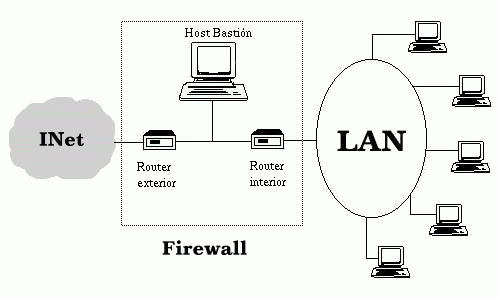
\includegraphics[width=\textwidth]{dmz.png}
\caption{Arquitectura DMZ.}
\label{dmz}
\end{center}
\end{figure}
\\Esta arquitectura de cortafuegos elimina los puntos \'unicos de fallo 
presentes en las anteriores: antes de llegar al basti\'on (por definici\'on, el
sistema m\'as vulnerable) un atacante ha de saltarse las medidas de seguridad 
impuestas por
el enrutador externo. Si lo consigue, como hemos aislado la m\'aquina basti\'on 
en una subred estamos reduciendo el impacto de un atacante que logre 
controlarlo, ya que antes de llegar a la red interna ha de comprometer 
tambi\'en al segundo {\it router}; en este caso extremo (si un pirata logra 
comprometer el segundo {\it router}), la arquitectura DMZ no es mejor que un 
{\it screened host}. Por supuesto, en cualquiera de los tres casos (compromiso
del {\it router} externo, del {\it host} basti\'on, o del {\it router} interno)
las actividades de un pirata pueden violar nuestra seguridad, pero de forma
parcial: por ejemplo, simplemente accediendo al primer enrutador puede aislar 
toda nuestra organizaci\'on del exterior, creando una negaci\'on de servicio 
importante, pero esto suele ser menos grave que si lograra acceso a la red
protegida.\\
\\Aunque, como hemos dicho antes, la arquitectura DMZ es la que mayores niveles
de seguridad puede proporcionar, no se trata de la panacea de los cortafuegos.
Evidentemente existen problemas relacionados con este modelo: por ejemplo, se 
puede utilizar el {\it firewall} para que los servicios fiables pasen 
directamente sin acceder al basti\'on, lo que puede dar lugar a un 
incumplimiento de la pol\'{\i}tica de la organizaci\'on. Un segundo problema,
quiz\'as m\'as grave, es que la mayor parte de la seguridad reside en los {\it
routers} utilizados; como hemos dicho antes las reglas de filtrado sobre 
estos elementos pueden ser complicadas de configurar y comprobar, lo que puede
dar lugar a errores que abran importantes brechas de seguridad en nuestro 
sistema.\\
\subsection{Otras arquitecturas}
Algo que puede incrementar en gran medida nuestra seguridad y al mismo tiempo
facilitar la administraci\'on de los cortafuegos es utilizar un basti\'on
diferente para cada protocolo o servicio en lugar de uno s\'olo; sin embargo,
esta arquitectura presenta el grave inconveniente de la cantidad de m\'aquinas
necesarias para implementar el {\it firewall}, lo que impide que muchas 
organizaciones la puedan adoptar. Una variante m\'as barata consistir\'{\i}a en
utilizar un \'unico basti\'on pero servidores {\it proxy} diferentes para
cada servicio ofertado.\\
\\Cada d\'{\i}a es m\'as habitual en todo tipo de organizaciones 
dividir su red en diferentes subredes; esto es especialmente aplicable en
entornos de I+D o empresas medianas, donde con frecuencia se han de conectar 
campus o sucursales separadas geogr\'aficamente, edificios o laboratorios 
diferentes, etc. En esta situaci\'on
es recomendable incrementar los niveles de seguridad de las zonas m\'as
comprometidas (por ejemplo, un servidor donde se almacenen expedientes o datos
administrativos del personal) insertando cortafuegos internos entre estas zonas
y el resto de la red. Aparte de incrementar la seguridad, {\it firewalls} 
internos son especialmente recomendables en zonas de la red desde la que no se
permite {\it a priori} la conexi\'on con Internet, como laboratorios de
pr\'acticas: un simple PC con Linux o FreeBSD que deniegue cualquier conexi\'on
con el exterior del campus va a ser suficiente para evitar que los usuarios 
se dediquen a conectar a p\'aginas {\it web} o {\it chats} desde equipos no
destinados a estos usos. Concretamente en el caso de redes de universidades 
ser\'{\i}a muy
interesante filtrar las conexiones a {\sc irc} o a {\sc mud}s, ya sea a nivel
de aulas o laboratorios o a nivel de todo el campus, denegando en el {\it 
router} de salida de la red hacia INet cualquier tr\'afico a los puertos 6667,
8888 y similares; aunque realmente esto no evitar\'{\i}a que todos los
usuarios siguieran jugando desde los equipos de la universidad -- por ejemplo 
a trav\'es de un servidor que disponga de conexi\'on en otros puertos --, 
s\'{\i} conseguir\'{\i}a que la mayor parte de ellos dejara de hacerlo.

\clearemptydoublepage
\chapter{PVM Y XPVM.}
\minitoc
\section{Introducci�n PVM.}
PVM (Paralel Virtual Machine) es una herramienta dise�ada para solucionarnos una gran cantidad de
problemas asociados con la programaci�n paralela. Sobre todo, el monetario. Para ello, nos va a crear una
nueva abstracci�n, que es la m�quina paralela virtual, empleando los recursos computacionales libres de
todas las m�quinas de la red que pongamos a disposici�n de la biblioteca. Es decir, disponemos de todas las
ventajas econ�micas asociadas a la programaci�n distribuida, ya que empleamos los recursos hardware de dicho
paradigma; pero programando el conjunto de m�quinas como si se tratara de una sola m�quina paralela, que es
mucho m�s c�modo.

La PVM es el est�ndar de facto del mundo cient�fico. De hecho, en el �rea de la F�sica Computacional,
la PVM es una biblioteca ampliamente usada.

La m�quina paralela virtual es una m�quina que no existe, pero un API apropiado nos permite programar como
si existiese. El modelo abstracto que nos permite usar el API de la PVM consiste en una m�quina multiprocesador
completamente escalable (es decir, que podemos aumentar y disminuir el n�mero de procesadores \textit{en caliente}).
Para ello, nos va a ocultar la red que estemos empleando para conectar nuestras m�quinas, as� como las
m�quinas de la red y sus caracter�sticas espec�ficas. Este planteamiento tiene numerosas ventajas respecto a
emplear un supercomputador, de las cuales, las m�s destacadas son:
\begin{itemize}
\item\textbf{Precio.} As� como es mucho m�s barato un computador paralelo que el computador tradicional
equivalente, un conjunto de ordenadores de mediana o baja potencia es much�simo m�s barato que el computador
paralelo de potencia equivalente. Al igual que ocurrir� con el caso del computador paralelo, van a existir
factores (fundamentalmente, la lentitud de la red frente a la velocidad del bus del computador paralelo) que
van a hacer de que sean necesarios m�s ordenadores de peque�a potencia que los te�ricos para igualar el
rendimiento. Sin embargo, aun teniendo esto en cuenta, la soluci�n es mucho m�s barata. Adem�s, al no ser la
PVM una soluci�n que necesite de m�quinas dedicadas (es decir, el \textit{daemon} de PVM corre como un proceso
m�s), podemos emplear en el proceso los tiempos muertos de los procesadores de todas las m�quinas de nuestra
red a las que tengamos acceso. Por ello, si ya tenemos una red Unix montada, el costo de tener un supercomputador
paralelo va a ser cero ya disponemos de las m�quinas, no tendremos que comprar nada nuevo, y adem�s la biblioteca
PVM es software libre, por lo que no hay que pagar para usarla.
\item\textbf{Disponibilidad}. Todo centro de c�lculo tiene un m�nimo de una docena de m�quinas
arrumbadas en una esquina, y que nadie sabe qu� hacer exactamente ya con ellas. Con esa docena que hace seis
a�os que ya no corren ni la �ltima versi�n del Word para Windows, podemos instalar Linux, la PVM y a�adirlo
al supercomputador paralelo virtual que conforma las m�quinas que ya tendr�amos en red.
\item\textbf{Tolerancia a fallos}. Si por cualquier raz�n falla uno de los ordenadores que conforman
nuestra PVM y el programa que la usa est� razonablemente bien hecho. Nuestra aplicaci�n puede seguir
funcionando sin problemas. En un caso como el nuestro, en el que la aplicaci�n va a estar corriendo durante
meses, es cr�tico que la aplicaci�n sea tolerante a fallos. Siempre hay alguna raz�n por la que alguna
m�quina puede fallar, y la aplicaci�n debe continuar haciendo los c�lculos con aquel hardware que contin�e
disponible.
\item\textbf{Heterogeneidad}. Podemos crear una m�quina paralela virtual a partir de ordenadores de
cualquier tipo. La PVM nos va a abstraer la topolog�a de la red, la tecnolog�a de la red, la cantidad de
memoria de cada m�quina, el tipo de procesador y la forma de almacenar los datos. Este �ltimo punto es de
extrema importancia, ya que el principal problema que tendr�amos en los \textit{sockets} era la programaci�n de
rutinas de conversi�n de formato de datos entre todos los ordenadores de la red, puesto que la codificaci�n,
tanto de enteros como de flotantes, puede ser distinta. Por �ltimo, nos permite incluir en nuestra PVM hasta
m�quinas paralelas. Una m�quina paralela en una PVM se puede comportar tanto como una sola m�quina secuencial
(caso, por ejemplo, del soporte SMP de Linux) o, como ocurre en muchas m�quinas paralelas, presentarse a la
PVM como un conjunto de m�quinas secuenciales.
\item\textbf{Disponibilidad}. La disponibilidad de la PVM es completa. La hemos encontrado con
facilidad para PowerPC con AIX, Sun con Solaris y PC 80x86 con Linux.
\end{itemize}
	
El uso de la PVM tiene muchas ventajas, pero tambi�n tiene una gran desventaja: nos podemos olvidar
del paralelismo fuertemente acoplado. Si disponemos de una red Ethernet, simplemente la red va a dejar de
funcionar para todas las aplicaciones (incluida PVM) de la cantidad de colisiones que se van a producir en
caso de que intentemos paralelismo fuertemente acoplado. Si disponemos de una red de tecnolog�a m�s avanzada;
es decir, m�s cara (como ATM) el problema es menor, pero sigue existiendo.

La segunda desventaja es que la abstracci�n de la m�quina virtual, la independencia del hardware y la
independencia de la codificaci�n tienen un coste. La PVM no va a ser tan r�pida como son los Sockets. Sin
embargo, si el grado de acoplamiento se mantiene lo suficientemente bajo, no es observable esta diferencia.

La arquitectura de la pvm se compone de dos partes. La primera parte es el daemon, llamado
\textit{pvmd}. En la versi�n actual de la PVM -la 3-, el nombre es \textit{pvmd3}. El daemon ha de estar
funcionando en todas las m�quinas que vayan a compartir sus recursos computacionales con la m�quina paralela
virtual. A diferencia de otros daemons y programas del sistema, el daemon de la PVM puede ser instalado por
el usuario en su directorio particular (de hecho, la instalaci�n por defecto es as�). Esto nos va a permitir
hacer supercomputaci�n como usuarios, sin tener que discutir con el administrador de la red que programas vamos
a poder ejecutar (aunque suele ser una buena idea comentar que vamos a instalar la PVM en el sistema, por la
carga que puede llegar a producir en las comunicaciones globales en algunos casos). Una vez que un usuario
(o superusuario) instal� en un directorio la PVM, todos los usuarios pueden hacer uso de esa instalaci�n con
el requisito de que el directorio donde est� instalada la PVM sea de lectura al usuario que quiera hacer uso
de ella.

En muchos centros de computaci�n, el administrador prefiere instalar �l mismo la PVM; con lo que,
adem�s de evitar que un usuario pueda borrarla sin consultar a los dem�s, va a permitir que todos los usuarios
tengan la PVM instalada por defecto; y, lo que es m�s importante, nosotros como administradores podremos
determinar el valor de \textit{nice} (prioridad del daemon) con el que va a ser lanzado el daemon pvmd3 y
as�, si este valor de nice es lo suficientemente alto, permite que la m�quina ejecute la PVM solamente en los
momentos ociosos.

Este daemon pvmd3 es el responsable de la m�quina virtual de por s�, es decir, de que se ejecuten
nuestros programas para la PVM y de gerenciar los mecanismos de comunicaci�n entre m�quinas, la
conversi�n autom�tica de datos y de ocultar la red al programador. Por ello, una vez que la PVM est� en
marcha, el paralelismo es independiente de la arquitectura de la m�quina, y s�lo depende de la arquitectura de
la m�quina virtual creada por la PVM. Esto nos va a evitar el problema que ten�amos con los Sockets ya que
ten�amos que hacer una rutina de codificaci�n y otra de decodificaci�n, al menos, por cada arquitectura
distinta del sistema.

Cada usuario, arrancar� el daemon como si de un programa normal se tratase, para ejecutar el c�digo
de PVM. Este programa se queda residente, realizando las funciones anteriores.

La segunda parte es la biblioteca de desarrollo. Contiene las rutinas para operar con los procesos,
transmitir mensajes entre procesadores y alterar las propiedades de la m�quina virtual. Toda aplicaci�n se ha
de enlazar a la biblioteca para poderse ejecutar despu�s. Tendremos tres ficheros de bibliotecas, la
\textit{libpvm3.a} (biblioteca b�sica en C), la \textit{libgpvm3.a} (biblioteca de tratamiento de grupos) y la
\textit{libfpvm3.a} (biblioteca para Fortran).

Un programa para PVM va a ser un conjunto de tareas que cooperan entre si. Las tareas se van a intercambiar
informaci�n empleando paso de mensajes. La PVM, de forma transparente al programador, nos va a ocultar las
transformaciones de tipos asociadas al paso de mensajes entre m�quinas heterog�neas. Toda tarea de la PVM puede
incluir o eliminar m�quinas, arrancar o parar otras tareas, mandar datos a otras tareas o sincronizarse con ellas.

Cada tarea en la PVM tiene un n�mero que la identifica un�vocamente, denominado \textbf{TID} (Task Identification Number).
Es el n�mero al que se mandan los mensajes habitualmente. Sin embargo, no es el �nico m�todo de referenciar
una tarea en la PVM. Muchas aplicaciones paralelas necesitan hacer el mismo conjunto de acciones sobre un
conjunto de tareas. Por ello, la PVM incluye una abstracci�n nueva, \textit{el grupo}. Un grupo es un conjunto
de tareas a las que nos podemos referir con el mismo c�digo, el identificador de grupo. Para que una tarea
entre o salga de un grupo, basta con avisar de la salida o entrada al grupo. Esto nos va a dotar de un
mecanismo muy c�modo y potente para realizar programas empleando modelos \textit{SIMD} (Single Instruction,
Multiple Data), en el que vamos a dividir nuestros datos en muchos datos peque�os que sean f�ciles de tratar,
y despu�s vamos a codificar la operaci�n simple y replicarla tantas veces como datos unitarios tengamos de
dividir el problema. Para trabajar con grupos, adem�s de enlazar la biblioteca de la PVM (\textit{libpvm3.a})
tenemos que enlazar tambi�n la de grupos (\textit{libgpvm3.a}).

Habitualmente para arrancar un programa para la PVM, se lanzar� manualmente desde un ordenador
contenido en el conjunto de m�quinas una tarea madre. La tarea se lanzar� con el comando \textit{spawn}
desde un monitor de la m�quina virtual, que a su vez se activar� con el comando pvm. Esta tarea se encargar�
de iniciar todas las dem�s tareas, bien desde su funci�n \textit{main} (que va a ser la primera en ejecutarse), bien desde alguna subrutina invocada por
ella. Para lanzar nuevas tareas se emplea la funci�n \textit{pvm{\_}spawn}, que devolver� un c�digo de error,
asociado a si pudo o no crearla, y el TID de la nueva tarea.

Para evitar el engorro de andar realizando transformaciones continuas de datos, la PVM define clases
de arquitecturas. Antes de mandar un dato a otra m�quina comprueba su clase de arquitectura. Si es la misma,
no necesita convertir los datos, con lo que se tiene un gran incremento en el rendimiento. En caso que sean
distintas las clases de arquitectura se emplea el protocolo XDR para codificar el mensaje.

Las clases de arquitectura est�n mapeadas en n�meros de codificaci�n de datos, que son los que
realmente se transmiten y, por lo tanto, los que realmente determinan la necesariedad de la conversi�n.

El modelo de paso de mensajes es transparente a la arquitectura para el programador, por la comprobaci�n
de las clases de arquitectura y la posterior codificaci�n con XDR de no coincidir las arquitecturas. Los
mensajes son etiquetados al ser enviados con un n�mero entero definido por el usuario, y pueden ser
seleccionados por el receptor tanto por direcci�n de origen como por el valor de la etiqueta.

El env�o de mensajes no es bloqueante. Esto quiere decir que el que env�a el mensaje no tiene que
esperar a que el mensaje llegue, sino que solamente espera a que el mensaje sea puesto en la cola de mensajes.
La cola de mensajes, adem�s, asegura que los mensajes de una misma tarea llegar�n en orden entre si. Esto no
es trivial, ya que empleando UDP puede que enviemos dos mensajes y que lleguen fuera de orden (UDP es un
protocolo no orientado a conexi�n). TCP, por ser un protocolo orientado a la conexi�n, realiza una reordenaci�n
de los mensajes antes de pasarlos a la capa superior, sin embargo, tiene el inconveniente que establecer las
conexiones entre nodos empleando TCP supone, si tenemos n nodos, tendremos un m�nimo de (\$n)(n\$-1) conexiones
TCP activas. Provocando esto que hasta para n�meros rid�culos de \$n\$ nos quedamos sin puertos por �ste
planteamiento. Establecer conexiones TCP entre procesos en lugar de entre nodos es peor todav�a, por las
mismas razones que en el caso de los nodos.

La comunicaci�n de las tareas con el daemon se hace empleando TCP. Esto se debe a que, al ser
comunicaciones locales, la carga derivada de la apertura y cierre de un canal es muy peque�o. Adem�s, no vamos
a tener tantas conexiones como en el caso de la conexi�n entre daemons, ya que las tareas no se conectan entre
s� ni con nada fuera del nodo, por lo que s�lo hablan directamente con su daemon. Esto determina que ser�n
\textit{n} conexiones TCP, que s� es una cifra razonable.

La recepci�n de los mensajes podemos hacerla mediante primitivas bloqueantes, no bloqueantes o con un
tiempo m�ximo de espera. La PVM nos dotar� de primitivas para realizar los tres tipos de recepci�n. En
principio nos ser�n m�s c�modas las bloqueantes, ya que nos dar�n un mecanismo de sincronizaci�n bastante
c�modo. Las de tiempo m�ximo de espera nos ser�n �tiles para trabajar con ellas como si fuesen bloqueantes,
mas dando soporte al hecho de que puede que el que tiene que mandarnos el mensaje se haya colgado. Por �ltimo,
la recepci�n de mensajes mediante primitivas no bloqueantes hace de la sincronizaci�n un dolor de cabeza. De
cualquier forma, en los tres casos anteriormente citados la misma PVM se encargar� de decirnos cu�ndo una
tarea acab�. Para informarnos de lo que pasa, emplea un mecanismo de eventos as�ncronos.

La PVM puede ser empleada de forma nativa como funciones en C y en C++, y como procedimientos en
Fortran. Basta para ello con tomar las cabeceras necesarias (si trabajamos con C o C++); y, para los tres,
enlazar con la biblioteca adecuada, que viene con la distribuci�n est�ndar. En el caso de C es libpvm3.a y en
el del Fortran \textit{libfpvm3.a}.

Si deseamos trabajar en otros lenguajes puede ser un poco m�s complejo. Si el lenguaje permite
incorporar funciones nativas en lenguaje C (como es el caso, por ejemplo, de Java) no hay ning�n problema;
ya que podemos invocar la funci�n; bien directamente si el lenguaje lo permite, bien haciendo alguna
peque�a rutina para adaptar el tipo de los datos, el formato de llamada a funci�n o cualquiera de las
restricciones que nos imponga el lenguaje que empleemos para invocar funciones en C.

Hemos de destacar que toda funci�n en C \textit{pvm{\_}alguna cosa} tiene como equivalente en Fortran
\textit{pvmfalgunacosa}, y viceversa.

El programa PVM corresponde al interprete de comandos de nuestra m�quina virtual. Algunos de los
comandos m�s importantes son:
\begin{itemize}
\item\textbf{add} m�quina: Incorpora la m�quina indicada a la m�quina paralela virtual.
\item\textbf{delete} m�quina: Elimina la m�quina indicada del conjunto de m�quinas asociadas a la
m�quina paralela virtual. Como es l�gico, no podremos eliminar la m�quina desde la que estamos ejecutando el
interprete de comandos.
\item\textbf{conf}: Configuraci�n actual de la m�quina paralela virtual.
\item\textbf{ps}: Listado de procesos de la m�quina paralela virtual. \textit{ps} -a lista todos los procesos.
\item\textbf{halt}: Apaga la m�quina paralela virtual. Esto significa que mata todas las tareas de
la PVM, elimina el daemon de forma ordenada y sale del programa pvm.
\item\textbf{help}: Lista los comandos del programa. Tremendamente �til en los momentos de desesperaci�n.
\item\textbf{id}: Imprime el TID de la consola.
\item\textbf{jobs}: Genera un listado de los trabajos en ejecuci�n.
\item\textbf{kill}: Mata un proceso de la PVM.
\item\textbf{mstat}: Muestra el estado de una m�quina de las pertenecientes a la PVM.
\item\textbf{pstat}: Muestra el estado de un proceso de los pertenecientes a la PVM.
\item\textbf{quit}: Sale de la m�quina paralela virtual sin apagarla.
\item\textbf{reset}: Inicializa la m�quina. Eso supone matar todos los procesos de la PVM salvo los programas monitores en ejecuci�n\'{o}n, limpiar
las colas de mensajes y las tablas internas y pasar a modo de espera todos
los servidores.
\item\textbf{setenv}: Lista todas las variables de entorno del sistema.
\item\textbf{sig} se�al tarea: Manda una se�al a una tarea.
\item\textbf{spawn}: Arranca una aplicaci�n bajo PVM. Es un comando bastante complejo cuyas opciones
veremos en una secci�n aparte.
\item\textbf{trace}: Actualiza o visualiza la m�scara de eventos traceados.
\item\textbf{alias}: Define un alias predefinido, es decir, un atajo para teclear un comando.
\item\textbf{unalias}: Elimina un alias predefinido.
\item\textbf{version}: Imprime la versi�n usada de la PVM.
\end{itemize}
Podemos obtener la PVM v�a ftp an�nimo: \url{ftp://netlib2.cs.utk.edu}

\section{Instalaci�n PVM.}
El paquete rpm de PVM que se va ha instalar es el que nos provee el cd de Red Hat Linux 6.2, para
llevar a cabo su instalaci�n se realizar� lo siguiente:
\begin{quote}
\textit{\$$>$mount /mnt/cdrom}\newline
\textit{\$$>$cd /mnt/cdrom/RedHat/RPMS/}\newline
\textit{\$$>$rpm --ivh pvm-3.4.3-4.i386.rpm}
\end{quote}
En el sitio web \url{http://www.epm.ornl.gov/pvm/pvm_home.html} se podr� obtener
la �ltima versi�n de dicho software adem�s de abundante informaci�n y sitios relacionados.

\section{Configuraci�n PVM.}
En el directorio del usuario se tendr� que crear la siguiente estructura de directorios
\textit{{\$}HOME/pvm3/bin/LINUX}. A continuaci�n se modificar� el archivo \textit{.bashrc} quedando de la siguiente forma:
\begin{em}
\begin{quote}
\textit{{\#} .bashrc}\newline
\textit{{\#} User specific aliases and functions}\newline
\textit{{\#} Source global definitions}\newline
\textit{if [ -f /etc/bashrc ]; then}\newline
\textit{. /etc/bashrc}\newline
\textit{fi}\newline
\textit{{\#} append this file to your .profile to set path according to machine}\newline
\textit{{\#} type. you may wish to use this for your own programs (edit the last}\newline
\textit{{\#} part to point to a different directory f.e. $\sim $/bin/{\_}{\$}PVM{\_}ARCH.}

\textit{export PVM{\_}ROOT=/usr/share/pvm3}\newline
\textit{export XPVM{\_}ROOT={\$}PVM{\_}ROOT/xpvm}

\textit{if [ -z {\$}PVM{\_}ROOT ]; then}\newline
\textit{if [ -d $\sim $/pvm3 ]; then} \newline
\textit{export PVM{\_}ROOT=$\sim $/pvm3}\newline
\textit{else}
\textit{print "Warning - PVM{\_}ROOT not defined"} \newline
\textit{print "To use PVM, define PVM{\_}ROOT and rerun your .profile"}
\textit{fi}
\textit{fi}

\textit{if [ -n {\$}PVM{\_}ROOT ]; then}\newline
\textit{export PVM{\_}ARCH=`{\$}PVM{\_}ROOT/lib/pvmgetarch`}\newline
\textit{{\#} uncomment one of the following lines if you want the PVM commands}\newline
\textit{{\#} directory to be added to your shell path.}\newline
\textit{export PATH={\$}PATH:{\$}PVM{\_}ROOT/lib {\#} generic}\newline
\textit{{\#} export PATH={\$}PATH:{\$}PVM{\_}ROOT/lib/{\$}PVM{\_}ARCH {\#} arch-specific}\newline
\textit{{\#} uncomment the following line if you want the PVM executable directory}\newline
\textit{{\#} to be added to your shell path.}\newline
\textit{export PATH={\$}PATH:{\$}PVM{\_}ROOT/bin/{\$}PVM{\_}ARCH}\newline
\textit{export PATH={\$}PATH:{\$}HOME/pvm3/bin/{\$}PVM{\_}ARCH} \newline
\textit{fi}
\end{quote}
\end{em}

A continuaci�n se crear� el archivo \textit{.pvmrc}, en el cual se incluir�n el nombre de los nodos
que van a formar la PVM. Dicho archivo tendr� la siguiente estructura:
\begin{em}
\begin{quote}
\textit{\# example PVM console startup script}\newline
\textit{\# copy this file to {\$}HOME/.pvmrc}\newline
\textit{\# command aliases}\newline
\textit{alias ? help}\newline
\textit{alias print{\_}environment spawn -> /bin/env}\newline
\textit{alias h help}\newline
\textit{alias j jobs}\newline
\textit{alias t ps}\newline
\textit{alias tm trace}\newline
\textit{alias v version}\newline
\textit{\# important for debugging}\newline
\textit{\#}\newline
\textit{setenv PVM\_EXPORT DISPLAY}\newline
\textit{\# want to see these trace events by default}\newline
\textit{tm addhosts delhosts halt}\newline
\textit{tm pvm\_mytid pvm\_exit pvm\_parent}\newline
\textit{tm send recv nrecv probe mcast trecv sendsig recvf}\newline
\textit{\#}\newline
\textit{\# inscripcion de los nodos que forman parte del cluster}\newline
\textit{\#}\newline
\textit{add pc1}\newline
\textit{add pc2}\newline
\textit{version \# print PVM release version}\newline
\textit{id \# print console TID}\newline
\textit{conf}
\end{quote}
\end{em}

Seguidamente se modificar� el fichero \textit{.rhosts} incluyendo el nombre de los nodos que van a
trabajar con la PVM.
\begin{em}
\begin{quote}
\textit{pc0 $ \to $ front end}\newline
\textit{pc1}\newline
\textit{pc2}
\end{quote}
\end{em}

\section{Compilaci�n y ejecuci�n de programas con PVM.}
Antes de compilar se tendr� que comprobar que la PVM esta activa de la siguiente forma:
\begin{em}
\begin{quote}
\textit{{\$}$>$pvm}
\end{quote}
\end{em}

Una vez activada la PVM utilizaremos el comando \textit{quit} para salir de esta.

Seguidamente se crear� un archivo llamado \textit{Makefile.aimk}, que tendr� la siguiente estructura:
\begin{em}
\begin{quote}
\textit{DEBUG = }\newline
\textit{SDIR = ..}\newline
\textit{BDIR = \$(HOME)/pvm3/bin}\newline
\textit{\#BDIR = \$(SDIR)/../bin}\newline
\textit{XDIR = \$(BDIR)/\$(PVM\_ARCH)} \newline
\textit{CC = gcc}\newline
\textit{OPTIONS = -g}\newline
\textit{CFLAGS= \$(OPTIONS) -I\$(PVM\_ROOT)/include \$(ARCHCFLAGS)}

\textit{LIBS = -lpvm3 \$(ARCHLIB)} \newline
\textit{GLIBS = -lgpvm3} \newline
\textit{LFLAGS= \$(LOPT) -L\$(PVM\_ROOT)/lib/\$(PVM\_ARCH) }

\textit{default: nombre\_programa -master nombre\_programa-slave}

\textit{nombre{\_}programa-master : {\$}(SDIR)/ejer5-master.c {\$}(XDIR)}newli
\textit{{\$}(CC) {\$}(DEBUG) {\$}(CFLAGS) -o {\$}@ {\$}(SDIR)/ejer5-master.c $\backslash $}\newline
\textit{{\$}(LFLAGS) {\$}(LIBS) -lm} \newline
\textit{cp {\$}@ {\$}(XDIR)}

\textit{nombre{\_}programa-slave : {\$}(SDIR)/nombre{\_}programa-slave.c {\$}(XDIR)}\newline
\textit{{\$}(CC) {\$}(DEBUG) {\$}(CFLAGS) -o {\$}@ {\$}(SDIR)/nombre{\_}programa-slave.c $\backslash $} \newline
\textit{{\$}(LFLAGS) {\$}(LIBS) -lm} \newline
\textit{cp {\$}@ {\$}(XDIR)}\newline
\textit{{\$}(XDIR):}\newline
\textit{- mkdir {\$}(BDIR)} \newline
\textit{- mkdir {\$}(XDIR)}

\textit{clean:}\newline
\textit{rm -f *.o nombre{\_}programa-master nombre{\_}programa-slave {\$}(XDIR)/nombre{\_}programa-master {\$}(XDIR)/ nombre{\_}programa -slave}\newline
\end{quote}
\end{em}
Para compilar los programas fuentes �nicamente se tendr� que hacer:
\textit{{\$}$>$ aimk}
\newline
En el caso de que se quiera borrar los c�digo objeto:
\begin{em}
\begin{quote}
\$$>$ \textit{aimk clean}
\end{quote}
\end{em}
Una vez que tenemos los programas ya compilados para ejecutarlos se realizar� lo siguiente:
\begin{em}
\begin{quote}
\$$>$ \textit{programa-master Numero de procesos}
\end{quote}
\end{em}
\section{Introducci�n XPVM}
En muchas ocasiones, es muy �til tener una representaci�n gr�fica de la configuraci�n de la m�quina
virtual que se est� utilizando, as� como una codificaci�n visual de la actividad llevada a cabo en cada host
de la m�quina virtual, qu� mensajes se est�n enviando, qui�n los env�a y a d�nde. La interfaz gr�fica de
usuario de PVM (XPVM) permite realizar todas estas funciones.

XPVM combina las funciones de la consola b�sica PVM con un monitor de seguimiento de actividades y un
debugger en una interfaz tipo X-Windows. XPVM est� escrito en C, usando el toolkit TCL/TK.

Para ejecutar XPVM, hay que asegurarse de que el daemon no est� ya corriendo y que no haya ficheros
temporales relacionados con PVM.

\begin{figure}[h!]
\begin{center}

\epsfig{file=imagenes/pvm/1.eps, width=3.75in}
\caption{Apariencia XPVM}
\end{center}
\end{figure}

Las consola se compone de varias vistas de tama�o reconfigurable y una serie de ventanas que son
utilizados por XPVM para mostrar mensajes de estado o de ayuda (Status y Help). Por defecto, la consola
inicialmente muestra la vista de red (Network View) y la vista de representaci�n temporal de tareas (Space-Time).

El men� Hosts nos permite a�adir un nuevo host a la m�quina virtual, seleccionado de entre todos los
hosts listados en el fichero \textit{.xpvm{\_}hosts}.

En este caso vamos a a�adir varios hosts. Cada vez que a�adimos uno aparece un nuevo s�mbolo de host
conectado a los s�mbolos existentes.

\begin{figure}[h!]
\begin{center}
\epsfig{file=imagenes/pvm/2.eps, width=3.75in}
\caption{Conexi�n entre nodos}
\end{center}
\end{figure}

A trav�s del men� Tasks-SPAWN pueden lanzarse tareas en cualquiera de los hosts que compone la m�quina.

La vista de Representaci�n de Tareas muestra el estado de todas las tareas que se est�n ejecutando en
la m�quina virtual en un momento dado. Para que las tareas se muestren, el bot�n PLAY que se ve en la parte
superior de la ventana de visualizaci�n de tareas. La visualizaci�n puede ser interrumpida o terminada en
cualquier momento, utilizando los botones PAUSE y STOP. Una vez detenida la visualizaci�n se mover hacia el
pasado o el futuro de las tareas utilizando los botones REWIND y FORWARD.

La vista de Representaci�n de Tareas se compone de dos ventanas. La ventana izquierda contiene el
nombre del host y el de la tarea ejecutada en el mismo. Las tareas aparecen ordenadas alfab�ticamente.
El n�mero de tareas mostradas en una ventana puede aumentarse utilizando el bot�n de compresi�n de tareas que
aparece a la izquierda de los botones anteriormente mencionados.

La ventana derecha muestra, para cada proceso, el estado de dicha tarea en cada momento, as� como
l�neas rojas que emanan de cada proceso y que corresponden a env�os de mensajes entre procesos. El c�digo de
colores muestra el estado del proceso, que puede estar ejecutando tareas propias (verde), rutinas PVM (amarillo)
o esperando mensajes (blanco).

\begin{figure}[h!]
\begin{center}
\epsfig{file=imagenes/pvm/3.eps, width=3.75in}
\caption{Representaci�n de las tareas}
\end{center}
\end{figure}

El usuario puede recabar informaci�n detallada sobre un estado determinado o un mensaje, seleccionando
con el bot�n izquierdo un estado u mensaje. Si se selecciona una barra de tarea, se obtiene su estado as� como
el tiempo de comienzo y fin de la tarea y la �ltima llamada a PVM que se hubiera generado. Si se selecciona una
l�nea de mensaje, la ventana que aparece mostrar� el tiempo de env�o y recepci�n, as� como el n�mero de bytes
enviado y el identificador de mensaje.

La representaci�n de tareas en la ventana derecha puede ampliarse o reducirse (zooming) utilizando
simult�neamente los dos botones del rat�n (simula el bot�n central de un rat�n de tres botones) y el
bot�n derecho, respectivamente.

Existe una ventana de salida de tareas, accesible a trav�s del men� VIEWS, que act�a como salida
standard para los procesos.

Finalmente, existe una ventana de utilizaci�n de recursos, accesible tambi�n a trav�s del men� VIEWS.
Esta ventana, que est� sincronizada con la ventana de representaci�n de tareas, muestra el n�mero de tareas
que est�n ejecut�ndose, ejecutando funciones PVM o en espera en cada momento.

\clearemptydoublepage
\chapter{LAM/MPI.}
\minitoc
\section{Introducci�n MPI.}
	El paso de mensajes es una tarea ampliamente usada en ciertas clases de m�quinas paralelas,
especialmente aquellas que cuentan con memoria distribuida. Aunque existen muchas variaciones, el concepto
b�sico en el proceso de comunicaci�n mediante mensajes es bien entendido. En los �ltimos 10 a�os, se ha
logrado un proceso substancial en convertir aplicaciones significativas hacia este tipo de tareas. M�s
recientemente diferentes sistemas han demostrado que un sistema de paso de mensajes puede ser implementado
eficientemente y con un alto grado de portabilidad.

	Al dise�arse MPI, se tomaron en cuenta las caracter�sticas m�s atractivas de los sistemas existentes
para el paso de mensajes, en vez de seleccionar uno solo de ellos y adoptarlo como el est�ndar. Resultando
as�, en una fuerte influencia para MPI los trabajos hechos por IBM, INTEL, NX/'', Express, nCUBE's Vernex,
p4 y PARMACS. Otras contribuciones importantes provienen de Zipcode, Chimp, PVM, Chameleon y PICL.

	La meta de MPI o Message Passing Interface (Interfaz de paso de mensajes), es el desarrollar un
est�ndar (que sea ampliamente usado) para escribir programas que implementen el paso de mensajes. Por lo cual
el interfaz intenta establecer para esto un est�ndar pr�ctico, portable, eficiente y flexible.

	El esfuerzo para estandarizar MPI involucro a cerca de 60 personas de 40 organizaciones diferentes
principalmente de U.S.A. y Europa. La mayor�a de los vendedores de computadoras concurrentes estaban involucrados
con MPI, as� como con investigadores de diferentes universidades, laboratorios del gobierno e industrias. El
proceso de estandarizaci�n comenz� en el taller de est�ndares para el paso de mensajes en un ambiente con
memoria distribuida, patrocinado por el Centro de Investigaci�n en Computaci�n Paralela en Williamsbur Virginia
(Abril 29-30 de 1992). Se llego a una propuesta preliminar conocida como \textit{MPI1}, enfocada principalmente
en comunicaciones punto a punto sin incluir rutinas para comunicaci�n colectiva y no presentaba tareas seguras. El
est�ndar final por el MPI fue presentado en la conferencia de Supercomputaci�n en Noviembre de 1993, constituy�ndose
as� el foro para el MPI.

	En un ambiente de comunicaci�n con memoria distribuida en la cual las rutinas de paso de mensajes de
nivel bajo, los beneficios de la estandarizaci�n son muy notorios. La principal ventaja al establecer un
est�ndar para el paso de mensajes es la portabilidad y el ser f�cil de utilizar.

	MPI es un sistema complejo, el cual comprende 129 funciones, de las cuales la mayor�a tiene muchos
par�metros y variantes.
	\newline
	
	\textbf{Metas del MPI}
	\begin{quote}
        \begin{itemize}
	\item Dise�ar una interfaz de programaci�n aplicable (no necesariamente para compiladores o sistemas que
implementan una librer�a).
        \item Permitir una comunicaci�n eficiente. Evitando el copiar de memoria a memoria y permitiendo (donde
sea posible) la sobreposici�n de computaci�n y comunicaci�n, adem�s de aligerar la comunicaci�n con el procesador.
	\item Permitir implementaciones que puedan ser utilizadas en un ambiente heterog�neo.
	\item Permitir enlaces convenientes en C y Fortran 77 para el interfaz.
        \item Asumir un interfaz de comunicaci�n seguro. El usuario no debe lidiar con fallas de comunicaci�n.
Tales fallas son controladas por el subsistema de comunicaci�n interior.
        \item Definir un interfaz que no sea muy diferente a los actuales, tales como PVM, NX, Express, p4, etc.,
y proveer de extensiones para permitir mayor flexibilidad.
        \item Definir un interfaz que pueda ser implementado en diferentes plataformas, sin cambios significativos
en el software y las funciones internas de comunicaci�n.
	\item La sem�ntica del interfaz debe ser independiente del lenguaje.
	\item La interfaz debe ser dise�ada para producir tareas seguras.
	\end{itemize}
	\end{quote}
	
\subsection{Modelo de programaci�n.}
        En el modelo de programaci�n MPI, un computo comprende de uno o m�s procesos comunicados a trav�s
de llamadas a rutinas de librer�as para mandar (send) y recibir (receive) mensajes a otros procesos. En la
mayor�a de las implementaciones de MPI, se crea un conjunto fijo de procesos al inicializar el programa, y un
proceso es creado por cada tarea. Sin embargo, estos procesos pueden ejecutar diferentes programas. De ah� que,
el modelo de programaci�n MPI es algunas veces referido como \textit{MPMD} (multiple program multiple data) para
distinguirlo del modelo \textit{SPMD}, en el cual cada procesador ejecuta el mismo programa.

	Debido a que el n�mero de procesos en un c�mputo de MPI es normalmente fijo, se puede enfatizar en el
uso de los mecanismos para comunicar datos entre procesos. Los procesos pueden utilizar operaciones de
comunicaci�n punto a punto para mandar mensajes de un proceso a otro, estas operaciones pueden ser usadas para
implementar comunicaciones locales y no estructuradas. Un grupo de procesos puede llamar colectivamente operaciones
de comunicaci�n para realizar tareas globales tales como broadcast, etc. La habilidad de MPI para probar
mensajes da como resultado el soportar comunicaciones as�ncronas. Probablemente una de las caracter�sticas
m�s importantes del MPI es el soporte para la programaci�n modular. Un mecanismo llamado comunicador permite
al programador del MPI definir m�dulos que encapsulan estructuras internas de comunicaci�n (estos m�dulos
pueden ser combinados secuencialmente y paralelamente).

\subsection{Bases.}
        Aunque MPI es un sistema complejo y multifac�tico, podemos resolver un amplio rango de problemas
usando seis de sus funciones, estas funciones inician y terminan un c�mputo, identifican procesos, adem�s de
mandar y recibir mensajes.
	\begin{itemize}
	\item\textbf{MPI\_INT:} Inicia un computo.\newline
MPI\_INT(int *argc,char ***argv), argc, argv son requeridos solo por el contexto del lenguaje C, en el cual
son los argumentos del programa principal.
        \item\textbf{MPI\_FINALIZE:} Termina un computo. MPI\_FINALIZE().
        \item \textbf{MPI\_COMM\_SIZE:} Determina el n�mero de procesos en un computo.  \newline
MPI\_COMM\_SIZE(comm,size), IN comm comunicador(manejador[handle]), \newline
OUT size n�mero de procesos en el grupo del comunicador(entero).
	\item\textbf{MPI\_COMM\_RANK:} Determina el identificador del proceso actual ``mi proceso''.\newline
MPI\_COMM\_RANK(comm,pid), IN comm comunicador (manejador[andel]), OUT pid identificador del proceso en el
grupo del comunicador(entero).
        \item\textbf{MPI{\_}SEND:} Manda un mensaje. MPI{\_}SEND(buf, count, datatype, dest, tag, comm). IN
buf direcci�n del buffer a enviar (tipo x), IN count n�mero de elementos a enviar del buffer (entero>=0), IN
datatype tipo de datos del buffer a enviar (handle), IN dest identificador del proceso destino (entero), IN
tag message tag (entero), IN comm comunicador (handle)
	\item\textbf{MPI{\_}RECV:} Recive un mensaje. MPI{\_}RECV(buf,count,datatype,dest,tag,comm). OUT buf
direcci�n del buffer a recibir (tipo x), IN count n�mero de elementos a recibir del buffer (entero>=0), IN
datatype tipo de datos del buffer a recibir (handle), IN source identificador del proceso fuente, o
MPI\_ANY\_SOURCE(entero), IN tag message tag, o MPI\_ANY\_TAG(entero), IN comm comunicador (handle), OUT status
estado del objeto (estado)
	\item\textbf{IN:} Significa que la funci�n usa pero no modifica el par�metro.
	\item\textbf{OUT:} Significa que la funci�n no usa pero puede modificar el par�metro.
	\item\textbf{INOUT:} Significa que la funci�n usa y modifica el par�metro.
        \end{itemize}
	Todas las funciones (excepto las dos primeras) toman un manejador (handle) ``comunicador'' como
argumento. El comunicador identifica el grupo de procesos y el contexto en el cual la operaci�n se debe
realizar. Como se menciono anteriormente, los comunicadores proveen un mecanismo para identificar subconjuntos
de procesos durante el desarrollo de programas modulares y para garantizar que los mensajes provistos con
diferentes prop�sitos no sean confundidos. Por ahora, es suficiente proveer el valor de default
MPI\_COMM\_WORLD, el cual identifica todos los procesos en un c�mputo.

	Las funciones MPI{\_}INT y MPI{\_}FINALIZE son usadas para iniciar y terminar un computo MPI,
respectivamente MPI\_INIT debe ser llamada antes que cualquier otra funci�n MPI y debe ser llamada solamente
una vez por proceso. Ninguna funci�n MPI puede ser llamada despu�s de MPI\_FINALIZE.

	Las funciones MPI\_COMM\_SIZE y MPI\_COMM\_BANK determinan el n�mero de procesos en el c�mputo actual
y el identificador (entero) asignado al proceso actual, respectivamente. Los procesos en un grupo de procesos
son identificados con un �nico y continuo n�mero (entero), empezando en 0.

	El est�ndar del MPI no especifica como un c�mputo paralelo es iniciado. Pero un mecanismo t�pico
podr�a ser el especificar desde la l�nea de comandos el n�mero de procesos a crear.
        \newline

	\textbf{Determinismo:}
        \begin{itemize}
	\item El paso de mensajes en m�dulos de programaci�n son por defecto no deterministicos; el orden de llegadas
de los mensajes enviados desde dos procesos A y B hacia un tercer proceso C, no esta definido. Pero, MPI
garantiza que dos mensajes enviados desde un proceso A, hacia otro proceso B, llegar�n en el orden en que
fueron enviados.
	\item En el modelo de programaci�n Tarea/Canal, el determinismo es garantizado al definir canales separados
para diferentes comunicaciones y al asegurar que cada canal tiene un solo escritor y un solo lector. Por lo
cual, un proceso C puede distinguir mensajes recibidos de A o B tal y como llegan en diferentes canales. MPI
no soporta canales directos, pero provee mecanismos similares; en particular, permite una operaci�n de recibimiento
para especificar una fuente, tag y/o contexto.
        \end{itemize}
	\textbf{Especificaciones en el contexto del lenguaje C:}
        \begin{itemize}
	\item Los nombres de las funciones son tal y como se presentan en la definici�n del MPI pero solo con el
prefijo de MPI y la primer letra del nombre de la funci�n en may�sculas.
        \item Los valores de los estados son regresados como c�digos enteros. El c�digo de regreso para una
ejecuci�n exitosa es MPI\_SUCESS.
	\item Tambi�n esta definido un conjunto de c�digos de error.
	\item Las constantes est�n en may�sculas y son definidas en el archivo mpi.h
	\item Los handles son representados por tipos especialmente definidos en mpi.h
	\item Los par�metros de las funciones del tipo IN son pasados por valor, mientras que los par�metros
OUT y INOUT son pasados por referencia (como apuntadores).
	\item Las variables de estado (status) tiene el tipo MPI\_Status y es una estructura con campos status.
MPI\_SOURCE y status.MPI\_TAG.
	\item Los tipos de datos del MPI est�n definidos para cada tipo de datos de C: MPI\_CHAR, MPI\_INT,
MPI\_LONG\_INT, MPI\_UNSIGNED\_CHAR, etc.
	\end{itemize}

\subsection{Operaciones globales.}
        Como ya se ha explicado, los algoritmos paralelos ejecutan llamadas a operaciones para coordinar la
comunicaci�n en m�ltiples procesos.
	Por ejemplo, todos los procesos pueden necesitar cooperar para invertir una matriz distribuida o para
sumar un conjunto de n�meros distribuidos en cada proceso. Claramente, estas operaciones globales pueden ser
implementadas por un programador usando las funciones send y receive. Por conveniencia y para permitir la
optimizaci�n, MPI provee un conjunto especializado de funciones colectivas de comunicaci�n que obtienen
operaciones de este tipo.

\subsection{Comunicaci�n as�ncrona.}
	La necesidad por tener una comunicaci�n as�ncrona puede presentarse cuando un computo necesita
acceder los elementos de un dato estructurado compartido en una manera no estructurada. Una implementaci�n
aproximada es el encapsular los datos estructurados en un conjunto de tareas de datos especializados, en la
cual las peticiones de lectura y escritura pueden ser ejecutadas. Este m�todo no es eficiente en MPI debido
a su modelo de programaci�n MPMD.

	Una implementaci�n alternativa con MPI, es el distribuir las estructuras de datos compartidas entre
los procesos existentes, los cuales deben solicitar peri�dicamente las solicitudes pendientes de lectura y
escritura. Para esto MPI presenta tres funciones MPI\_IPROBE, MPI{\_}PROBE, MPI{\_}GET{\_}COUNT.
	\begin{itemize}
	\item\textbf{MPI\_IPROBE:} chequea existencia de mensajes pendientes sin recibirlos, permiti�ndonos
escribir programas que generan c�mputos locales con el procesamiento de mensajes sin previo aviso. El mensaje
puede ser recibido usando MPI\_RECV.
	\item\textbf{MPI\_PROBE:} es utilizado para recibir mensajes de los cuales se tiene informaci�n
incompleta. El siguiente fragmento de c�digo hace uso de estas funciones para recibir un mensaje de una fuente
desconocida y con un n�mero de enteros desconocidos como contenido. Primero detecta la llegada del mensaje
utilizado MPI\_PROBE. Despu�s, determina la fuente del mensaje y utiliza \textbf{MPI{\_}GET{\_}COUNT} para
conocer el tama�o del mensaje.Finalmente, direcciona un buffer par recibir el mensaje.
        \end{itemize}
\subsection{Modularidad.}

	Conocemos ya tres formas generales de composici�n que puede ser usadas en la construcci�n modular de
programas paralelos, a saber, secuencial, paralelo y concurrente.

	MPI soporta la programaci�n modular a trav�s de su mecanismo de comunicador (comm, el cual provee la
informaci�n oculta necesaria al construir un programa modular), al permitir la especificaci�n de componentes
de un programa, los cuales encapsulan las operaciones internas de comunicaci�n y proveen un espacio para el
nombre local de los procesos.

	Una operaci�n de comunicaci�n MPI siempre especifica un comunicador. Este identifica el grupo de
procesos que est�n comprometidos en el proceso de comunicaci�n y el contexto en el cual la comunicaci�n ocurre.
El grupo de procesos permite a un subconjunto de procesos el comunicarse entre ellos mismos usando identificadores
locales de procesos y el ejecutar operaciones de comunicaci�n colectivas sin meter a otros procesos. El contexto
forma parte del paquete asociado con el mensaje. Una operaci�n \emph{receive} puede recibir un mensaje solo si este fue
enviado en el mismo contexto. Si dos rutinas usan diferentes contextos para su comunicaci�n interna, no puede
existir peligro alguno en confundir sus comunicaciones.

	A continuaci�n se describen las funciones que permiten a los comunicadores ser usados m�s flexiblemente.
        \begin{itemize}
        \item\textbf{MPI\_COMM\_DUP:} Un programa puede crear un nuevo comunicador, conteniendo el mismo grupo
de procesos pero con un nuevo contexto para asegurar que las comunicaciones generadas para diferentes prop�sitos
no sean confundidas, este mecanismo soporta la composici�n paralela.
	\item\textbf{MPI\_COMM\_SPLIT:} Un programa puede crear un nuevo comunicador, conteniendo solo un subconjunto
del grupo de procesos. Estos procesos pueden comunicarse entre ellos sin riesgo de tener conflictos con otros
c�mputos concurrentes. Este mecanismo soporta la composici�n paralela.
	\item\textbf{MPI\_INTERCOMM\_CREATE:} Un programa puede construir un intercomunicador, el cual enlaza
procesos en dos grupos. Soporta la composici�n paralela.
	\item\textbf{MPI\_COMM\_FREE:} Esta funci�n puede ser utilizada para liberar el comunicador creado al usar
funciones anteriores.
        \end{itemize}
\subsection{Instalaci�n.}
        El paquete rpm de LAM/MPI que se va ha instalar es el que nos provee el cd de Red Hat Linux 6.2, para llevar
a cabo su instalaci�n se realizar� lo siguiente:
	\begin{quote}
		\textit{{\$}$>$mount /mnt/cdrom}\newline
                \textit{{\$}$>$cd /mnt/cdrom/RedHat/RPMS/}\newline
                \textit{{\$}$>$rpm --ivh lam-6.3.1-4.i386.rpm}
	\end{quote}
	En el sitio web \url{http://www.lam-mpi.org/download/} se podr� obtener la �ltima versi�n de dicho
software.

\subsection{Configuraci�n.}
	En el directorio \textit{/usr/boot} crearemos los siguiente archivos con sus correspondientes
configuraciones.
        \begin{enumerate}
	\item Archivo conf.lam, se recoger� la topolog�a de red utilizada.
        \begin{quote}\textit{lamd \$inet\_topo}\end{quote}
       	\item Archivo bhost.def, se a�adir� al final los nombres de todos los nodos que forman parte del cluster.
       	\begin{em}
	\begin{quote}
		localhost
		pc1
		pc2
		\ldots
	\end{quote}
	\end{em}
        \end{enumerate}
        Para testear si la configuraci�n es correcta se deber� de realizar lo siguiente:

        \begin{quote}\textit{{\$}$>$lamboot}\end{quote}
        Si la salida muestra alg�n error entonces es que hay alg�n problema con la instalaci�n, comunicaci�n
 entre nodos, etc.

\section{Compilaci�n y ejecuci�n de programas LAM/MPI}
	Se generar� el siguiente fichero llamado \textit{makefile}, que tendr� la siguiente estructura:
	\begin{em}
      	\begin{quote}
      		.SILENT: \newline
		CFLAGS=-I/usr/include/lam -L/usr/lib/lam \newline
		CC=mpicc \newline
		nombre{\_}programa : nombre{\_}programa.c
		\$(CC) \$(CFLAGS) nombre\_programa.c -o nombreprograma
	\end{quote}
	\end{em}
	Para compilar los programas LAM/MPI se utilizar� el siguiente comando:
	
	\begin{quote}\textit{\$$>$make -f makefile}\end{quote}
	
	Una vez compilado el programa y antes de ejecutarlo se necesitar� primero arrancar el sistem Multicomputador
de Area Local, esto se hace a trav�s del comando \textit{lamboot}.

	Para ejecutar el programa se utilizar� el siguiente comando:
	
	\begin{quote}\textit{\$$>$mpirun --np n$^{o}$ de procesos nombre\_programa argumentos}\end{quote}


\clearemptydoublepage
\chapter{BWATCH. HERRAMIENTA SOFTWARE PARA OBSERVAR EL ESTADO DEL CLUSTER.}
\minitoc
\section{Introducci�n.}
La herramienta \textit{bWatch 1.0.3} es un peque�o programa TCL/TK, el cual muestra en una ventana un conjunto de
informaci�n a cerca de cada uno de los nodos que conforma el cluster, es decir, es un sistema de monitorizaci�n del
cluster.

La informaci�n que nos prove� dicho software es:

\begin{itemize}
\item Host name.
\item N� de usuarios conectados.
\item Hola en la cual se hizo la toma de los datos.
\item Carga hace 1 min.
\item Carga hace 5 min.
\item Carga hace 15 min.
\item Numero de procesos.
\item Memoria total.
\item Memoria libre.
\item Memoria compartida.
\item Buffers.
\item Cache.
\item Total de swap.
\item Swap libre.
\end{itemize}

La �ltimas versiones de este software est�n disponibles en \url{ftp://www.sci.usq.edu.au/pub/jacek/bWatch/}.

bWatch puede ser ejecutado por cualquier usuario mientras �ste pueda ejecutar RSH (Remote Shell) en todas las
m�quinas que conforman el cluster.

bWatch fue desarrollado para plataformas LINUX.

\section{Instalaci�n.}
Una vez descargado el software \textit{bWatch-1.0.3.tar.gz} se descomprime en el directorio de usuario
\textit{\$HOME} y se compila. A continuaci�n se muestra la secuencia de pasos a realizar:
\begin{em}
\begin{quote}
\$$>$/home/usuario/\newline
\$$>$tar -xvfz bWatch-1.0.3\newline
\$$>$cd /home/usuario/bWatch-1.0.3 \newline
\$$>$make bWatch $\Rightarrow$ \textit{genera un ejecutable llamado bWatch.tcl}\newline
\$$>$make install $\Rightarrow$ \textit{inserta bWatch en} /usr/local/bin
\end{quote}
\end{em}
	
\section{Configuraci�n.}
Se editar� el fichero \textit{\$HOME/.bWatchrc.tcl} y en la sentencia \textit{set listOfHosts} se incluir� el
nombre de los nodos que conforman el cluster
\begin{em}
\begin{quote}
set bWatchrcVersion 1.0.0\newline
set listOfHosts {pc0 pc1}

\# set the columns which should be displayed\newline
\# 1 - information will be displayed for every host\newline
\# 0 - column will not be shown

\# number of users on the system\newline
set display(numUsers) 1\newline
\# system time\newline
set display(time) 1\newline
\# 1 minute averga load\newline
\#set display(load1) 1\newline
\# 5 minutes average load\newline
set display(load5) 1\newline
\# 15 minutes average load\newline
set display(load15) 1\newline
\# number of processes\newline
set display(numProcesses) 1\newline
\# total RAM\newline
set display(totalMemory) 1

\# available free RAM\newline
set display(freeMemory) 1\newline
\# shared RAM\newline
set display(sharedMemory) 1\newline
\# buffered memory\newline
set display(buffers) 1\newline
\# cached memory\newline
set display(cache) 1\newline
\# total swap space\newline
set display(totalSwap) 1\newline
\# available swap space\newline
set display(freeSwap) 1

\# foreground and background coulours\newline
\# of the heading of the table\newline
set colour(headingBG) \#066\newline
set colour(headingFG) \#FFF

\# foreground and background colours\newline
\# of the first column showing host names   \newline
set colour(hostNameBG) \#006\newline
set colour(hostNameFG) \#FFF

set colour(neutralFG) black \newline
set colour(firstWarningFG) orange   \newline
set colour(secondWarningFG) \#A00\newline
set colour(errorFG) \#F00\newline
set colour(errorBG) \#FFF

set loadLimit(firstWarning) 1.5\newline
set loadLimit(secondWarning) 2.5\newline
set loadLimit(error) 5.0

set freeMemLimit(firstWarning) 1024\newline
set freeMemLimit(secondWarning) 512\newline
set freeMemLimit(error) 1

set freeSwapLimit(firstWarning) 20480\newline
set freeSwapLimit(secondWarning) 10240\newline
set freeSwapLimit(error) 5120\newline
set blank -------\newline
set cell(width) 8
\end{quote}
\end{em}
La herramienta bWatch obtiene los resultados de los distintos nodos a trav�s del protocolo RSH,
por lo tanto, en el fichero \textit{\$HOME/.rhosts} deber�n estar incluidos los nombres de los nodos que conforman
el cluster. Un ejemplo podr�a ser:
\begin{em}
\begin{quote}
pc0\newline
pc1\newline
\ldots
\end{quote}
\end{em}

\section{Visualizaci�n del estado del cluster.}
Para poder visualizar el estado se realizar� lo siguiente:
\begin{em}
\begin{quote}
\$$>$cd \$HOME/bWatch-1.0.3\newline
\$$>$./bWatch.tcl
\end{quote}
\end{em}
A continuaci�n nos aparecer� la siguiente tabla en la cual podremos observar el estado de cada uno de los nodos
que conforma el cluster

\begin{figure}[h!]
\begin{center}
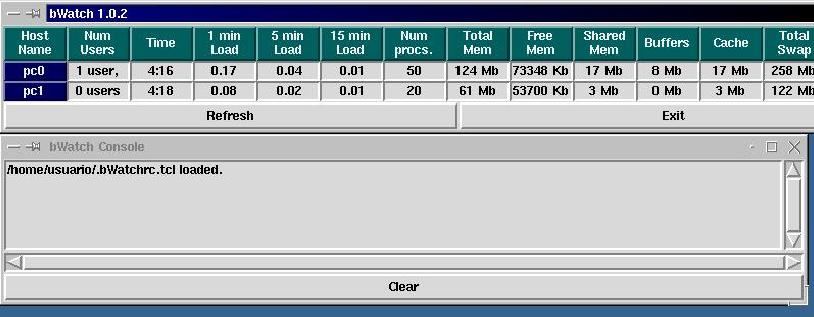
\epsfig{file=imagenes/bWatch/bWatch.eps, width=4.25in}
\caption{Monitorizaci�n Cluster}
\end{center}
\end{figure}
\clearpage
\clearemptydoublepage

%\chapter{Bibliografia}
\begin{thebibliography}{9}
\bibitem{bib-PS} Javier Garc�a de Jal�n, Iker Aguinaga, Alberto Mora
\emph{Aprenda Linux como si estuviese en primero}
San Sebastian (Espa�a), 2000
\bibitem{Julian Lopez Ruise�o}
\emph{Linux: Instalaci�n y Primeros Pasos. Version 2.2.2}
Madrid (Espa�a), 1996
\bibitem {Gerhard Mourani}
\emph{Securing and Optimizing Linux: RedHat Edition}
Lion (Francia), 2000
\bibitem{Antonio Villal�n Huerta}
\emph{Seguridad en UNIX y redes}
Madrid (Espa�a), 1999
\bibitem{}
\emph{Gu�a de Administraci�n de Redes con Linux}, 2000
\bibitem{Diego Berea Cabaleiro, Juan Jos� S�nchez Penas}
\emph{Seguridad De Redes Corporativas Basada En Firewall II}
\bibitem{\emph{Firewall How-To Document For Linux}}
\bibitem{\emph{Firewall scripts} http://www.linuxdoc.org/LDP/solrhe/Securing-Iptimizing-Linux-RH-Edition-v.13/fwall-scripts.html}
\bibitem{\emph{Gu�a De Seguridad Del Administrador De Linux} http://athena.fit.qut.edu.au/linux/networks.html}
\bibitem{\emph{DHCP How-To Document For Linux}}
\bibitem{\emph{Instalaci�n y Configuraci�n DHCP} http://www.geocities.com/linux2005/documentos/servidordhcpd.htm}
\bibitem{\emph{Diskless, Remote-Boot Linux} http://www.physics.ohio-state.edu/~clkim/system/linux-farm.html}
\bibitem{\emph{PVM 3 User's Guide and Reference Manual Date Published. 1994}}
\end{thebibliography}
\end{document}
